%\documentclass[fleqn]{article}
\documentclass[msc,numbers, fleqn]{coppe}
\renewcommand\thesection{\arabic{section}}
\usepackage[utf8]{inputenc}
\usepackage{hyperref}
\usepackage{indentfirst}
\usepackage{empheq}
%\usepackage{mathptmx}
\usepackage{amsmath}
\usepackage{amssymb}
\usepackage{gensymb}
\usepackage{commath}
\usepackage{cancel}
\usepackage{tikz}
\usepackage{bm}
\usepackage{siunitx}
\usepackage{tcolorbox}
\usepackage{pgfplots}
\usepackage{filecontents}
\usepackage{natbib} 
\usepackage{graphicx}
\usepackage{setspace}
\usepackage[font=small, labelfont=bf]{caption}
\usepackage{enumerate}
\usepackage{nccmath}
\usepackage{booktabs}
\usepackage{multirow}
\usepackage{wasysym}
\usepackage{xcolor}
%\usepackage{kantlipsum}
\setcitestyle{authoryear,round, sort}
\usepackage[nottoc]{tocbibind}
%\captionsetup[figure]{font={stretch=1.5}}
\usetikzlibrary{shapes.geometric,calc}
\pgfplotsset{compat=1.4}
% \addtolength{\oddsidemargin}{-.875in}
% \addtolength{\evensidemargin}{-.875in}
% \addtolength{\textwidth}{1.75in}
% 
% \addtolength{\topmargin}{-.875in}
% \addtolength{\textheight}{1.75in}
\pgfplotsset{compat=newest} % Allows to place the legend below plot
\usepgfplotslibrary{units} % Allows to enter the units nicely
\renewcommand{\baselinestretch}{1.5}

\allowdisplaybreaks

\setcounter{secnumdepth}{5}

\numberwithin{figure}{section}
\numberwithin{table}{section}
\numberwithin{equation}{section}

\makelosymbols
\makeloabbreviations

\begin{document}

\abbrev{SI}{Sistema Internacional de Unidades}
\abbrev{RTC}{Resistência térmica de contato}
\abbrev{CTC}{Condutância térmica de contato}
\abbrev{IHTP}{\textit{Inverse Heat Transfer Problem} -- Problema Inverso de Transferência de Calor}

\symbl{$\mathbb{R}$}{Conjunto dos n\'umeros reais}

\title{Um método analítico para estimativa
de condutâncias térmicas de contato em interfaces irregulares usando a
técnica da Transformada Integral Clássica e o método dos funcionais de reciprocidade}
\foreigntitle{An analytical method for estimation of thermal contact conductances on irregular interfaces using the generalized integral transform technique
and the reciprocity functional method}
  \author{Guilherme}{Camelo de Freitas}
  \advisor{Prof.}{Marcelo José}{Colaço}{D.Sc.}
  \examiner{Prof.}{Nome do Primeiro Examinador Sobrenome}{D.Sc.}
  \examiner{Prof.}{Nome do Segundo Examinador Sobrenome}{Ph.D.}
  \department{PEM}
  \date{\month}{\the\year}
  
  \keyword{Problemas Inversos}
  \keyword{Funcional de Reciprocidade}
  \keyword{Condutância Térmica de Contato}
  \keyword{Transformada Integral}
 
 \maketitle
 
 \frontmatter
  \dedication{À Ludmilla, minha esposa, minha companheira, minha amiga, meu alicerce. Te amo!}
  
  \chapter*{Agradecimentos}
  
  Agradeço a Deus, pois em todo tempo é bom.
  
  À Petrobras, pela oportunidade oferecida.
  
  À minha esposa Ludmilla, que sempre esteve ao meu lado em todo esse processo. Dedico este trabalho a você.

  Ao meu gerente imediato, Roberto Gonçalves, por proporcionar condições adequadas que permitiram a conclusão deste trabalho.
  
  Ao professor Marcelo Colaço, pela orientação e paciência, e sobretudo pela confiança.
  
  Ao professor Renato Cotta, que me apresentou a técnica da Transformação Integral Clássica.
  
  Aos meus colegas de trabalho e amigos Daniel Fialho e Andreia Carvalho, pelo apoio e compreensão durante o período de desenvolvimento deste trabalho.
  
  Ao meu colega de trabalho e amigo Elísio Caetano Filho, pelo incentivo a não desistir.
  
  Aos meus colegas de trabalho e amigos Eduardo Gaspari, Carlos Dittz e Ricardo Minette, pelas sugestões e trocas de ideias.
  

 
 \begin{abstract}
 
O método dos funcionais de reciprocidade, aliado à Técnica da Transformada Integral Clássica (CITT), tem sido aplicado com sucesso na obtenção de
soluções analíticas para o problema inverso de transferência de calor que procura estimar a distribuição da condutância térmica de contato (CTC) ao longo da interface plana
de um corpo constituído de dois materiais. O desenvolvimento teórico sobre o qual esta abordagem se baseia, contudo, não está limitado à necessidade de que esta
interface tenha um formato regular.

Este trabalho propõe estender o método, obtendo assim um desenvolvimento analítico para estimativa da distribuição da condutância térmica de contato em interfaces não necessariamente
regulares. Para tanto, algumas ferramentas serão empregadas, a saber: a extensão do domínio físico irregular num domínio físico regular sobre o qual os
problemas auxiliares serão resolvidos analiticamente; e a aplicação do processo de ortogonalização de Gram-Schmidt para gerar um conjunto ortonormal
de funções a partir das soluções obtidas pelos problemas auxiliares.


  \end{abstract}
  
  \begin{foreignabstract}

The reciprocity functional method, associated to the Classic Integral Transform Technique (CITT), has been succesfully applied in obtaining analytical
solutions for the inverse heat transfer problem that seeks to estimate the thermal contact conductance (TCC) distribution on the interface of a body composed of
two materials. Yet, the theoretical development upon which this approach is based is not limited to the need of this interface to have a regular format.

This work proposes to extend the method, thus obtaining an analytical development for the estimation of the thermal contact conductance distribution on interfaces which
are not necessarily regular. Therefore, some tools will be employed, namely: the extension of the irregular physical domain to a regular physical domain in
which the auxiliary problems will be analytically solved; and the application of the Gram-Schmidt orthogonalization process in order to generate an orthonormal set
of functions from the solutions obtained from the auxiliary problems.
 
  \end{foreignabstract}

\tableofcontents
 \listoffigures
 \listoftables
 \printlosymbols
 \printloabbreviations

  \mainmatter
  
\section{Introdução}

\subsection{Motivação}

Quando há transferência de calor através da fronteira comum entre dois corpos materiais em contato físico, observa-se experimentalmente que nessa interface há
uma descontinuidade no perfil de temperatura, ou seja, o contato térmico nessa região não é perfeito \citep{livro_ozisik}. 
Esse fenômeno ocorre devido à combinação dos efeitos de três componentes \citep{livro_madhusudana}:
\begin{itemize}
  \item Condução de calor através dos pontos em que há contato efetivo sólido-sólido, devido à presença de irregularidades microscópicas e macroscópicas;
  \item Condução de calor através do meio intersticial, preenchido por algum fluido (por exemplo, ar);
  \item Radiação de calor, que é desprezada na maioria das aplicações. 
\end{itemize} 


% 
% Na maioria das aplicações, os efeitos de radiação são desprezados, bem como  Mesmo a altas pressões, o fenômeno da descontinuidade de temperatura permanece relevante, pois a
% superfície efetiva de contato não coincide com a superfície total de contato.

A figura \ref{fig1} ilustra o processo de transferência de calor através da interface de contato entre dois sólidos. As linhas de fluxo de calor
sofrem uma \textit{constrição} nos pontos de contato, e uma maior dispersão nos espaços entre os pontos.

\begin{figure}[h!b]
\begin{center}
\begin{tikzpicture}
\node at (0, 0)
	{
		\includegraphics[trim=250 642 150 154, clip=true]{img/img1.pdf}
	};
	
\node[scale=0.8] at (0, 0.9) {Sólido 1};
\node[scale=0.8] at (0, -1.1) {Sólido 2};
\node[scale=0.8] at (4, 0.3) {Fluido};
%\node[scale=0.8] at (-5.5, 0.05) {Interface de contato \Gamma};
\end{tikzpicture}
\caption{Transferência de calor através da interface entre dois corpos (adaptado de \citeauthor{livro_ozisik}, \citeyear{livro_ozisik})}
\label{fig1}
\end{center}
\end{figure}

A \textit{condutância térmica de contato} -- abreviada como CTC -- é definida como sendo a razão entre o fluxo de calor e o salto de temperatura
devido à presença do contato imperfeito \citep{livro_madhusudana}:
\begin{equation}
	h_c = \frac{Q_c/A}{\Delta T_c} = \frac{q_c}{\Delta T_c} \label{eq:definicao_1}
\end{equation}
onde $Q_C$ é o fluxo total de calor através da interface, $A$ é a área de contato nominal ou aparente, $q_c$ é o fluxo de calor por unidade de área e e $\Delta T_c$ é o salto de temperatura na interface. As unidades
da CTC são as mesmas do coeficiente de transferência de calor por convecção (W/($\text{m}^2$ K) no SI).

A inversa da CTC é denominada \textit{resistência térmica de contato} (RTC):
\begin{equation}
	R_c = \frac{1}{h_c} = \frac{A\Delta T_c}{Q_c} = \frac{\Delta T_c}{q_c}
\end{equation}

Uma definição equivalente da CTC pode ser formulada a partir da análise do problema de condução de calor no domínio constituído pelos
corpos em contato, através das condições de contorno avaliadas na interface de contato \citep{livro_ozisik}. Nessa região, pode-se afirmar que o fluxo
de calor saindo ou entrando em cada um dos sólidos deve se igualar ao fluxo de calor através da interface.

Sejam, portanto, $T_1$ e $T_2$ os campos de temperatura em cada um dos sólidos cuja interface, designada pelo símbolo $\Gamma$, é representada na figura \ref{fig1}. Sejam $k_1$ e $k_2$
as respectivas condutividades térmicas dos sólidos, e seja $q_c$ o fluxo de calor por unidade de área através da interface de contato. Assim, o balanço de energia permite escrever:
\begin{equation}
	q_c = -k_1\frac{\partial T_1}{\partial \mathbf{n}_1}\bigg|_\Gamma
	=
	h_c(T_1 - T_2)_\Gamma
	=
	k_2\frac{\partial T_2}{\partial \mathbf{n}_2}\bigg|_\Gamma \label{eq:definicao_2}
\end{equation}
De onde se obtém:
\begin{equation}
	h_c = \frac{-k_1\displaystyle\frac{\partial T_1}{\partial \mathbf{n}_1}\bigg|_\Gamma}{(T_1 - T_2)_\Gamma} = \frac{k_2\displaystyle\frac{\partial T_2}{\partial \mathbf{n}_2}\bigg|_\Gamma}{(T_1 - T_2)_\Gamma} \label{eq:definicao_3}
\end{equation}
Os gradientes de temperatura são calculados sobre as direções dos vetores normais
$\mathbf{n}_1$ e $\mathbf{n}_2$, que apontam para fora das fronteiras que delimitam os corpos materiais correspondentes; em particular,
na interface de contato teremos $\mathbf{n}_2 = -\mathbf{n}_1$.

Nota-se facilmente a partir da equação \eqref{eq:definicao_3} que a CTC é uma propriedade não necessariamente constante ao longo da interface de contato,
uma vez que tanto o fluxo de calor como o salto entre as temperaturas podem variar em cada ponto sobre a interface. De fato, nos locais onde a diferença é nula (ou seja, o contato
é perfeito), a CTC assumiria valor infinito, ou alternativamente, a RTC seria nula. No outro extremo, havendo uma região micrométrica perfeitamente
isolante entre os corpos materiais, o fluxo de calor seria nulo para uma diferença de temperatura finita; ali a CTC seria nula, equivalente a um valor
infinito de RTC. Assim, a CTC também pode ser entendida como um parâmetro de avaliação da qualidade do contato entre dois corpos materiais.

O levantamento da CTC também permite avaliar qualitativamente a presença de descontinuidades ou falhas
em materiais homogêneos, uma vez que, devido aos saltos de temperatura provocados pela interface de contato no local da falha,
o campo de temperatura medido na superfície externa fornece resultados diferentes do esperado se tais falhas não ocorressem.

A necessidade de cálculo ou estimativa da CTC se faz presente em diversas aplicações, como por exemplo, na área aeroespacial \citep{artigo_aerospacial}, microeletrônica
\citep{artigo_snaith}, ou no projeto de trocadores de calor \citep{artigo_huang}. Para tanto, podem ser aplicados métodos de medição que normalmente exigem
algum conhecimento de detalhes das superfícies de contato, tais como rugosidade ou aspereza, e necessitam de tomadas de temperatura no interior dos corpos em contato, levando a arranjos
experimentais complexos ou intrusivos. Conhecidas (ou estimadas por regressão) as temperaturas na interface e o fluxo de calor por unidade de área, a aplicação
direta da definição permite levantar a CTC, normalmente como um valor médio sobre a interface. Essa foi a abordagem adotada na maioria dos problemas de estimativa
de CTC registrados na literatura.

O problema da estimativa da CTC tem características que permitem classificá-lo como um problema inverso de transferência de calor (IHTP, do termo em inglês
\textit{Inverse Heat Transfer Problem}). Num problema direto de transferência de calor, conhecem-se as propriedades termofísicas dos materiais envolvidos, a geometria do domínio, 
a taxa de geração de calor e as
condições de contorno e inicial; através desses parâmetros se obtém a distribuição de temperaturas no domínio de interesse. Já o problema inverso procura
estimar algum dos parâmetros (ou funções, caso haja variação espacial e/ou temporal da propriedade que se deseja estimar) relacionados previamente, utilizando medidas de temperatura em um ou mais pontos do domínio \citep{livro_beck_2}.
Nesse contexto, a CTC se enquadra como uma propriedade termofísica passível de ser estimada através da resolução de um IHTP. Uma grande vantagem dessa
abordagem é a possibilidade de tratar a CTC como uma propriedade distribuída espacialmente ao longo da interface de contato, ou seja, uma função da posição sobre a interface; por outro lado, problemas
inversos são bastante sensíveis a erros de medição dos dados de entrada. Algumas estratégias podem ser aplicadas
a fim de contornar essas dificuldades, como por exemplo a técnica de regularização de Tikhonov \citep{livro_tikonov}.

O tratamento da estimativa da CTC como um problema inverso de transferência de calor não eliminou a necessidade de se ter disponíveis as medições de
temperatura na interface de contato. A determinação indireta da distribuição dessas temperaturas sobre a interface, através de métodos não intrusivos,
tem sido objeto de pesquisas recentes, levando ao desenvolvimento de técnicas de estimativa de CTC mais eficientes computacionalmente
\citep{artigo_colaco_1, artigo_colaco_2, artigo_colaco_3, artigo_colaco_4, artigo_padilha_3}. Tais técnicas, porém, têm sido aplicadas em configurações
físicas e geométricas regulares, tais como interfaces de contato planas ou de seção transversal circular, o que simplifica consideravelmente o tratamento
analítico-numérico do problema inverso de transferência de calor, em detrimento de uma maior abrangência em resolver problemas de estimativa de CTC
envolvendo geometrias menos comuns.

\subsection{Objetivo}

O objetivo principal desta dissertação é, através de uma abordagem analítico-numérica, estudar o problema da estimativa da CTC entre superfícies
de dois corpos materiais colocados em contato, considerando o fato de que tais superfícies não são necessariamente regulares.  

O ponto de partida foi o trabalho desenvolvido por \cite{tese_padilha}, que estudou o problema da estimativa da CTC numa superfície
plana entre dois corpos materiais colocados em contato. O problema-teste analisado foi configurado de forma que a seção transversal do
conjunto composto pelos dois
corpos materiais tivesse formato retangular e a CTC sobre a interface dependesse
espacialmente de apenas uma coordenada cartesiana. O referido trabalho forneceu uma expressão analítica que estima de forma direta
o perfil de CTC ao longo do comprimento da interface. Para resolução do problema inverso que fornecia a CTC, foram empregadas as técnicas dos Funcionais de Reciprocidade \citep{artigo_andrieux},
e da Transformação Integral Clássica (CITT) \citep{livro_cotta}. Este resultado representou uma contribuição inédita aos estudos de levantamento de perfil de CTC,
ao introduzir um método direto, não iterativo, de baixo custo computacional e que não emprega medidas intrusivas de temperatura no interior dos corpos em contato.

Ao se acompanhar o desenvolvimento analítico envolvendo o uso da técnica dos Funcionais de Reciprocidade, nota-se que as expressões obtidas, basicamente integrais de contorno, não dependiam necessariamente de
alguma geometria particular de seção transversal dos corpos materiais, ou da interface de contato, ou mesmo do sistema de coordenadas empregado.
Contudo, as características geométricas do problema-teste original permitiram que o emprego da CITT simplificasse consideravelmente estas integrais.

Para desenvolver esta dissertação, foi feita uma modificação na configuração geométrica do problema-teste: a interface de contato entre os corpos passou a
ter uma forma curvilínea, representada por uma equação da forma $y = w(x)$, mantendo-se o formato retangular na seção transversal do conjunto
de teste. Assim, a interface plana estudada por \cite{tese_padilha} passou a ser um caso particular do problema abordado no presente trabalho, para
o qual $w(x) = \text{constante}$. Essa alteração introduziu complexidades ao problema que, num primeiro momento, eliminariam as vantagens computacionais
proporcionadas pelo emprego da CITT, e que foram contornadas através do uso de conceitos e ferramentas clássicas da Álgebra Linear e de uma redefinição conveniente
do domínio geométrico do problema.

\subsection{Organização do trabalho}

O presente capítulo introduziu a definição formal de condutância térmica de contato e apresentou os conceitos e ferramentas básicas a serem aplicados ao longo do trabalho (a saber, os Funcionais de Reciprocidade e a Técnica da Transformada Integral Clássica). Os fatores motivacionais e os objetivos principais da dissertação também foram apresentados.

No capítulo 2 é apresentada uma revisão bibliográfica descrevendo separadamente a evolução das técnicas de solução de problemas difusivos e as abordagens do tratamento da estimativa da condutância térmica de contato, desenvolvendo ambos os aspectos pelo ponto de vista histórico.

O capítulo 3 apresenta a descrição do problema físico abordado neste estudo. A configuração física, que consiste basicamente em um corpo de prova de seção reta retangular feito de dois materias distintos em contato, foi estabelecida levando-se em conta que a interface de contato entre os materiais pode ser representada por uma curva. As hipóteses assumidas e a formulação matemática do problema de condução de calor, em que a CTC aparece como um dos dados de entrada, são indicados neste capítulo.

O capítulo 4 descreve o problema inverso de condução de calor referente ao arranjo físico estabelecido no capítulo 3, no qual a CTC passa a ser uma função a ser estimada. Neste arranjo, assume-se que as medidas de temperatura na superfície superior do corpo de prova são conhecidas. O conceito de Funcional de Reciprocidade é descrito neste capítulo, bem como a sua formulação proposta para o problema estudado. Conceitos matemáticos de Álgebra Linear necessários para o embasamento teórico da técnica dos Funcionais de Reciprocidade, tais como espaços lineares, produtos internos e projeções ortogonais, também são discutidos.

No capítulo 5 são formulados os problemas difusivos auxiliares que fornecem as funções auxiliares necessárias para o cálculo dos Funcionais de Reciprocidade. Uma vez que a interface de contato entre os materiais que compõem o corpo de prova não é plana nem horizontal, faz-se necessário aplicar conceitos de Geometria Diferencial para expressar em coordenadas cartesianas o gradiente de temperatura ao longo da interface, que aparece nas condições de contorno dos problemas auxiliares. Desse modo, é feita uma adequação da formulação dos problemas para permitir a aplicação da Técnica da Transformada Integral Clássica para sua solução; todo o processo de resolução através desta ferramenta é detalhado neste capítulo. As funções obtidas são então ortogonalizadas através do algoritmo de Gram-Schmidt.

Os resultados obtidos nos capítulos anteriores são reunidos no capítulo 6, onde finalmente é apresentada a formulação analítica da estimativa da condutância térmica de contato. Mais uma vez são revisitadas ferramentas de Geometria Diferencial, quais sejam, integrais de linha e derivadas direcionais, que auxiliam na formalização das conceitos estabelecidos ao longo do trablho. A expressão final proposta é de propósito geral, para interfaces de contato de formato arbitrário, sendo a interface plana horizontal, que inspirou o presente trabalho, um caso particular.

Discussões sobre a implementação numérico-computacional da estimativa da condutância térmica de contato, bem como os resultados numéricos obtidos pela aplicação da metodologia, têm lugar no capítulo 7. Foram executadas simulações computacionais de diferentes configurações de geometria de interface de contato e de condutância térmica de contato, a fim de obter as medidas simuladas de temperatura na superfície superior dos corpos de prova. Estas medidas por sua vez alimentaram um programa escrito em Fortran, que implementa as equações deduzidas até o capítulo anterior, fornecendo as respectivas estimativas de condutância térmica de contato. Os resultados teóricos e estimados foram comparados e as análises correspondentes foram desenvolvidas ao longo deste capítulo.

A dissertação se encerra no capítulo 8, onde são apresentadas conclusões quanto ao emprego da técnica dos Funcionais de Reciprocidade no problema inverso estudado e indica sugestões de trabalhos futuros para a continuidade do desenvolvimento desta técnica.

\section{Revisão bibliográfica}

A revisão bibliográfica exposta nesta seção está dividida em duas partes. Na primeira parte, é feito um levantamento sobre a evolução histórica
das técnicas de solução de problemas difusivos, uma vez que, conforme será visto nos próximos capítulos, o problema inverso de condução de calor
a partir do qual será estimada a CTC é um problema difusivo. Na segunda parte, é apresentado um apanhado dos trabalhos clássicos que envolvem o tema da
determinação da CTC, antes e depois da introdução da abordagem deste tema como um problema inverso.

\subsection{Técnicas de soluções de problemas difusivos}

Segundo \cite{livro_tanehill}, há basicamente três abordagens ou métodos que podem ser usados para resolver um problema
de mecânica dos fluidos e/ou transferência de calor: experimental, teórico (ou analítico) e computacional (ou numérico). O primeiro
fornece resultados mais realistas a um custo de implementação maior. Já o segundo faz suposições
simplificadoras a fim de facilitar o tratamento do problema, e possivelmente encontrar uma solução fechada, ou seja, que é expressa geralmente como uma fórmula
matemática; uma vez que não envolve iterações ou interpolações, a obtenção do valor da solução num determinado ponto do domínio é praticamente imediata,
com baixo custo computacional. No último método -- a abordagem numérica -- as equações que governam o fenômeno em estudo são substituídas por
esquemas numéricos, cuja solução (obtida através de cálculos manuais ou pelo emprego de computadores digitais) é usada para representar de forma
aproximada a solução do problema original.

A teoria matemática moderna sobre a condução de calor foi estabelecida por Joseph Fourier, que reuniu suas investigações teóricas em sua obra
\textit{Théorie analytique de la chaleur} \citep{livro_fourier, artigo_langer}. Neste trabalho, Fourier deduz analiticamente as equações de condução para vários
tipos de sólidos, como esferas, prismas retangulares ou cilindros de seção reta circular. Nesses problemas, o fluxo de calor tinha
sempre uma direção que favorecia o aspecto simétrico do sólido em questão; por exemplo, no caso do cilindro ou da esfera, o fluxo
de calor acontecia na direção radial. Em seguida, Fourier apresenta a formulação tridimensional em coordenadas cartesianas da equação
de condução de calor em regime transiente, e a emprega para levantar as equações obtidas previamente, através de substituições de
variáveis. Finalmente, Fourier desenvolve o conceito de representação de uma função como um somatório infinito de funções
trigonométricas\footnote{A história registra que, quando Fourier apresentou seus artigos sobre a representação de funções arbitrárias
como expansões de senos e cossenos à Academia de Ciências de Paris em 1807 e 1811, recebeu críticas dos consultores (principalmente Lagrange,
que negou veementemente essa possibilidade), devido à falta de rigor, e por isso os artigos não foram publicados \citep{livro_agarwal}.} e, através da aplicação
da técnica de separação de variáveis, usa esse conceito na resolução analítica dos problemas que propôs no início do trabalho. Uma vez que os domínios envolvidos e as
condições de contorno impostas nos problemas possuíam algum tipo de simetria, que simplificava a variação da temperatura para apenas uma
variável dimensional (distância radial, comprimento ao longo de um eixo, etc.), as soluções encontradas eram relativamente simples, o que não
diminui sua importância por modelarem matematicamente o fenômeno físico da condução de calor pela primeira vez. O tratamento
dado por Fourier aos problemas de condução de calor foi, em suma, predominantemente analítico, sem considerações de caráter numérico.

Historicamente, os livros acadêmicos que versam sobre transferência de calor reproduzem a dedução da equação de condução em coordenadas
cartesianas feita por Fourier e em seguida apresentam a formulação equivalente nos sistemas de coordenadas cilíndricas e esféricas; ver
por exemplo \cite{livro_carslaw}, \cite{livro_holman} e \cite{livro_ozisik}. De fato, a formulação no sistema cartesiano é aplicável
a qualquer tipo de geometria; a solução geral sempre poderá ser expressa em termos de somatórios de senos ou cossenos. Soluções analíticas obtidas
nos sistemas de coordenadas esféricas ou cilíndricas envolvem somatórios de tipos diferentes de funções base ortogonais, obtidas através da aplicação do método
de separação de variáveis \citep{livro_boyce}. Voltando a citar os trabalhos de Fourier, ao expressar
as equações de condução para corpos esféricos ou cilíndricos, ele fez implicitamente um \textit{mapeamento} dessas geometrias a partir
do sistema de coordenadas cartesiano para os sistemas de coordenadas cilíndricas ou esféricas \citep{livro_numerical_grid}, e, ao aplicar a
separação de variáveis, encontra soluções em forma de séries que futuramente seriam associadas às funções de Bessel e Legendre \citep{livro_fourier}. 

\cite{artigo_einsenhart, artigo_einsenhart_2} demonstrou que a equação de Helmholtz (da qual a equação
de difusão é um caso particular) pode ser resolvida por separação de variáveis em onze diferentes
sistemas de coordenadas ortogonais, dentre as quais figuram os sistemas cartesiano, esférico e cilíndrico, bem como outros menos usuais, tais
como elíptico-cilíndrico ou parabólico. \cite{livro_moon} fizeram um extenso levantamento das equações diferenciais ordinárias
oriundas da separação de variáveis em cada um desses sistemas, e apresentam suas respectivas soluções gerais (dentre as quais estão as funções
seno e cosseno e as funções de Bessel e Legendre, já citadas). Tais equações, juntamente com as respectivas condições de contorno, constituem-se
em \textit{problemas de valor de contorno de Sturm-Liouville} \citep{artigo_sturm, artigo_liouville}. Problemas de Sturm-Liouville são na realidade
parte de uma teoria fundamental da Álgebra Linear conhecida como teoria dos operadores lineares; isto confere características e propriedades
especiais às soluções desses problemas (denominadas \textit{autofunções}), tais como a ortogonalidade e a possibilidade de, sob certas condições, expressar uma função arbitrária
como uma combinação linear dessas autofunções \citep{livro_boyce, livro_axler}.

Os métodos numéricos de solução de equações diferenciais ganharam grande impulso a partir da década de 1960, quando houve uma maior disponibilidade
de computadores digitais de alto desempenho \citep{livro_tanehill}. Aliado a esse fato, houve também um aumento natural da complexidade dos problemas de transferência
de calor e mecânica dos fluidos: adoção de geometrias complexas ou não convencionais, formulações de condições de contorno que introduziam dificuldades na
aplicação dos métodos analíticos, menores restrições quanto a não linearidade dos problemas. Já as abordagens numéricas, contudo, remontam a épocas anteriores. 

Uma dessas abordagens, considerada pioneira na análise numérica de equações diferenciais parciais em problemas
difusivos, foi proposta por \cite{artigo_richardson}. Em seu artigo, Richarsdon resolve numericamente a equação de Laplace e a equação biarmônica, e aplica esta última no problema prático de estudo da distribuição de tensão numa
barragem de alvenaria, com uma geometria bidimensional. Para tanto, ele representa o perfil da barragem usando segmentos de reta e emprega uma malha estruturada regular em seu interior. A malha
era resolvida usando um esquema iterativo de diferenças finitas centradas \citep{livro_tanehill}. Richardson já destacava as limitações dos métodos analíticos na integração de equações diferenciais parciais nos casos em que as fronteiras têm formato irregular.

Os anos seguintes testemunharam uma grande quantidade de pesquisas em mé-todos numéricos, especialmente no campo dos problemas de dinâmica dos fluidos. Avanços na área dos
problemas difusivos envolvem técnicas de precondicionamento de sistemas lineares e o desenvolvimento de esquemas de sobrerrelaxação, aumentando significativamente
o desempenho da taxa de convergência da solução \citep{artigo_frankel, artigo_fedorenko}.

Em meados da década de 1970, sistemas de coordenadas generalizadas, coincidentes com as fronteiras de domínios irregulares,
começam a ser empregados em detrimento dos sistemas de coordenadas ortogonais convencionais na resolução numérica de problemas advectivos-difusivos,
com o objetivo de evitar interpolações entre pontos da malha não coincidentes com as fronteiras \citep{livro_maliska}. As fronteiras do domínio físico, definidas geralmente no sistema 
cartesiano, são mapeadas para uma região retangular no domínio computacional, definido no sistema de coordenadas generalizado, através de relações de transformação.

A distribuição dos pontos na malha estruturada do problema físico original é feita de modo que a malha correspondente no domínio computacional seja regular. 
As equações diferenciais e as condições de contorno devem ser reescritas nesse novo sistema; as equações resultantes são mais complicadas uma vez que contêm mais
termos e coeficientes variáveis. Tais equações podem ser discretizadas e resolvidas usando, por exemplo, a técnica das diferenças finitas aplicada à malha retangular definida no domínio computacional.
Finalmente, a solução é transformada de volta para o domínio físico através das relações de transformação. Destaca-se o trabalho de \citet{artigo_thompson},
que desenvolveram uma técnica para determinação da relação de transformação entre sistemas de coordenadas para o caso bidimensional através da resolução numérica de equações diferenciais parciais.

Outra técnica de transformação de coordenadas envolve o emprego de transformações conformes \citep{livro_numerical_grid}. Uma grande vantagem
dessa técnica é o fato de que a equação de difusão preserva a forma original, sem introdução de termos não-lineares ou derivadas cruzadas;
por outro lado é aplicável apenas a geometrias bidimensionais. Se as fronteiras da geometria do problema não tiverem uma descrição algébrica
conhecida, também deve se fazer uso de esquemas de geração numérica de malha, baseados por exemplo na transformação de Schwarz-Christoffel \citep{livro_brown}.

Voltando ao trabalho de Fourier, é possível identificar em seu trabalho uma das bases sobre a qual se estabeleceu a técnica analítica de solução
de equações diferenciais parciais conhecida como transformação integral. No tratado previamente citado \textit{Théorie analytique de la chaleur},
procurando estender suas ideias para funções definidas em intervalos infinitos, Fourier descobriu uma fórmula de transformação integral e
sua respectiva inversa, que hoje levam o seu nome \citep{livro_integral_transforms}.

A técnica da transformação integral revelou-se uma
ferramenta poderosa para resolver problemas de valor inicial e problemas de valor de contorno para equações diferenciais parciais lineares.
O conceito de transformação integral originou-se dos trabalhos de Laplace, que publicou os primeiros resultados envolvendo a sua transformada
no tratado de 1812, \textit{Théorie analytique des probabilités} \citep{livro_integral_transforms}. Cauchy publicou em 1843 uma descrição
dos métodos simbólicos ou operacionais (que trabalham com operadores diferenciais como se fossem algébricos) \citep{livro_cauchy} e sua relação com a transformada de
Laplace, além de apresentar a forma exponencial da transformada de Fourier. Contudo, quem popularizou o uso das transformadas de Laplace foi Oliver Heaviside,
aplicando-as na resolução de equações diferenciais lineares em problemas de circuitos elétricos, especialmente a equação do telégrafo, consolidando as bases do
cálculo operacional moderno \citep{livro_yavetz, artigo_carson}. 

A grande vantagem oferecida pela transformação integral aplicada às equações de difusão linear é a possibilidade de resolver analiticamente classes de
problemas para os quais a técnica de separação de variáveis não é adequada.
No caso específico das equações de difusão linear, as transformações integrais procuram reduzir a quantidade de variáveis independentes
na equação original, geralmente levando a uma nova equação diferencial ordinária de fácil solução. Exemplos elementares de aplicação
de transformação integral em problemas difusivos nos sistemas cartesiano e cilíndrico foram apresentados por \cite{artigo_doetsch}, \cite{artigo_sneddon} e \cite{livro_tranter},
e em coordenadas esféricas por \cite{artigo_olcer}.
\cite{livro_unified} classificaram e revisaram sete classes de problemas difusivos lineares, apresentando suas soluções
exatas obtidas pela técnica da transformação integral, que por razões históricas passou a ser denominada Técnica da Transformação Integral Clássica (CITT).

A CITT não se mostrou flexível o suficiente para fornecer
soluções analíticas para tipos de problemas mais gerais. Nesse sentido, o trabalho desenvolvido por \cite{artigo_murray},
que tratava problemas difusivos transientes com coeficientes variáveis nas condições de contorno, foi pioneiro no desenvolvimento da técnica
que é conhecida hoje como Transformada Integral Generalizada (GITT) \citep{livro_integral_transforms_cotta}. Desde então, a GITT --- uma técnica
híbrida analítico-numérica --- vem sido continuamente desenvolvida e estendida, fornecendo soluções analíticas aproximadas e numéricas alternativas
para os problemas não solucionáveis pela abordagem clássica. Nos últimos anos, a GITT tem sido beneficiada e popularizada através do desenvolvimento de
aplicativos de \textit{software} de computação simbólica, especialmente o \textit{Mathematica}\textsuperscript{\textregistered} \citep{artigo_mathematica}.

A técnica de transformação integral, seja clássica ou generalizada, é formulada com base em integrais sobre um domínio cuja
fronteira não é necessariamente regular. Em muitos casos, a transformação integral foi empregada em problemas difusivos ou advectivo-difusivos nos quais a geometria
era irregular, porém descrita de forma algébrica no sistema de coordenadas cartesiano, como por exemplo os trabalhos de \cite{artigo_aparecido, artigo_aparecido_2, artigo_aparecido_3, artigo_fausto} e \cite{artigo_perez}.
Já \cite{tese_sphaier} generaliza as técnicas de levantamento de autofunções nestes trabalhos e apresenta uma solução formal para domínios irregulares usando GITT;
para fronteiras cuja descrição algébrica é desconhecida, Sphaier sugere aproximar por linhas poligonais (no caso bidimensional), em que cada
trecho é representado por um segmento de reta. As autofunções levantadas no processo de solução são obtidas a partir de problemas auxiliares resolvidos no próprio
domínio irregular do problema, e nesse caso diz-se que o domínio é \textit{coincidente}; é feita uma rápida citação sobre soluções de problemas difusivos em domínios \textit{envolventes}
(quando o domínio original é considerado como sendo contido por um domínio maior, regular, sobre o qual a solução geral é encontrada e então particularizada
para aquele subdomínio).

As soluções da equação de difusão em dutos de seção reta elíptica com condições de contorno de primeiro e segundo tipo encontradas por
 \citet{trabalho_maia_1, trabalho_maia_2} combinaram as técnicas de transformação integral e mapeamento conforme. 
Isto se seguiu com \cite{tese_antonini}, que usa a mesma metodologia em sua dissertação de mestrado sobre resolução de problemas difusivo-convectivos em geometrias não-convencionais (setor circular, geometria anular
concêntrica e geometria bicônica). Conforme citado anteriormente, as equações de difusão no novo sistema de coordenadas preservaram sua forma; isso facilitou em
muito o emprego da GITT, uma vez que os problemas de autovalor associado geraram funções seno e cosseno. Por outro lado, a
simplificação nas soluções analíticas ou híbridas encontradas só foi possível porque as geometrias envolvidas possuíam mapeamentos conformes de expressão analítica
conhecida \citep{livro_brown}.

Recentemente, houve o aumento do interesse na aplicação de métodos numéricos \textit{meshless} na resolução
de problemas difusivos em geometrias irregulares; tais métodos procuram superar as dificuldades computacionais envolvidas na geração
de malhas de discretização, trabalhando com o conceito de nós distribuídos pelo domínio do problema, e com as interações entre nós
vizinhos. Tais técnicas incluem, por exemplo, o emprego de redes neurais \citep{artigo_deng, artigo_heidari}, funções de base
radial associadas ao método de colocação \citep{artigo_chen, artigo_dai}, o método SPH (\textit{smoothed particle hydrodynamics}) \citep{artigo_vishwakarma} e o método MLPG (\textit{Meshless Local Petrov-Galerkin})
\citep{artigo_li}.



\subsection{Estimativa da condutância térmica de contato}

No tratado sobre funções de Bessel escrito por \cite{livro_bessel}, são deduzidas soluções para problemas de propagação de ondas e de fluxo de
eletricidade que envolvem essas funções. No início do capítulo XII, os autores afirmam que é possível fazer uma analogia entre os problemas
elétricos desenvolvidos no texto com problemas de condução de calor, desde que se relacione, por exemplo, o potencial elétrico com a temperatura. Algumas
dessas análises teóricas levam em conta a resistência elétrica na região de contato entre dois materiais, considerando a existência de um fino
estrato nessa região. Os autores pressupõem a presença de uma descontinuidade de potencial elétrico entre as superfícies,
que seria função da resistividade do material do estrato, e resolvem analiticamente o problema difusivo de potencial elétrico nessa região de pequena espessura. 
Com base nisso, \cite{tese_mikic} afirma que, ainda de forma indireta, as primeiras análises teóricas sobre o fluxo de calor através de superfícies
em contato remontam à época de publicação desse trabalho. Mesmo assim, os primeiros estudos efetivos acerca da estimativa da CTC eram basicamente experimentais,
e foram impulsionados por necessidades nas áreas de projeto de reatores nucleares e na indústria aeroespacial \citep{tese_mikic}.

\cite{artigo_fenech} apresentam um modelo
teórico de CTC, baseado na hipótese de o contato entre as superfícies metálicas acontecer em apenas em alguns pontos, cuja distribuição superficial
é uniforme, e desprezando o fluxo de calor
nas regiões de vazios. A expressão analítica da CTC encontrada depende principalmente de três parâmetros: número de pontos de contato por unidade
de área, altura média dos vazios e razão entre área efetiva de contato e área total. Esses parâmetros são obtidos a partir de medidas tomadas nas
interfaces individuais, com auxílio de um perfilômetro. Os autores comparam os resultados teóricos com observações experimentais, e observam que,
a baixas pressões, a CTC se aproxima da condutividade térmica do fluido que preenche os vazios da interface. É importante observar que neste trabalho
e nos seguintes, a CTC é calculada como um valor único e constante sobre a superfície de contato.

Uma situação especialmente interessante para a área aeroespacial é o estudo da CTC em ambientes no vácuo. Este caso foi examinado por \cite{artigo_clausing}.
Em seu modelo, os autores distinguem os efeitos de constrição microscópica e macroscópica, e afirmam que estes últimos têm influência preponderante
na resistência térmica de contato. Tambem comentam sobre o efeito da chamada ``resistência de filme'', causado, por exemplo, pela presença de
filmes de óxidos em superfícies metálicas, e que podem apresentar influência significativa em ambientes no vácuo, sendo normalmente desprezados
nas análises em que há fluido presente no interstício. São definidos dois parâmetros adimensionais, baseados nas características geométricas e
físicas dos materiais, a partir dos quais é definida a CTC. 

\cite{tese_mikic} levantou expressões analíticas para resistências térmicas nos pontos de contato entre corpos metálicos, havendo presença de
fluido ou em ambiente de vácuo. Em seguida, fez uma descrição do perfil de rugosidade das superfícies de contato
a partir da distribuição gaussiana de probabilidade, a fim de determinar o número de contatos por unidade de área. Finalmente, relacionou a área efetiva de 
contato com a pressão aplicada sobre os materiais. Efeitos de filme foram desprezados, de forma a considerar apenas os efeitos de constrição.
Neste trabalho, a fase experimental, para fins de comparação com o modelo teórico, envolveu o emprego de um analisador de superfície para registrar os perfis de superfície, a partir dos quais foram obtidos
os desvios-padrão das amplitudes das rugosidades. A concordância entre os valores de CTC calculados e medidos foi, em geral, satisfatória; ainda assim,
para o caso de fluidos de baixa condutividade térmica, os valores de CTC previstos pelo modelo foram maiores do que os obtidos através dos experimentos. 

Uma investigação do efeito da difusão de calor em regime transiente na CTC foi conduzida por \cite{artigo_beck}. Nesse artigo, os campos de temperatura são
calculados separadamente para cada um dos dois corpos em contato, e medidas de temperatura são tomadas em pontos não necessariamente próximos da interface
de contato. A estimativa da CTC é a que miminiza o erro quadrático médio entre as temperaturas medidas e calculadas nesses pontos, avaliado em cada instante
discreto de tempo em que são feitas as medições.

Vários experimentos envolvendo fluidos diferentes na interface entre os corpos em contato, e sua influência na CTC, foram realizados por \cite{artigo_madhusudana}.
Considerações teóricas não foram feitas nesse trabalho. O autor mostra empiricamente que a presença de um meio condutor de calor na interface melhora a CTC,
especialmente a baixas pressões e se o meio for um bom condutor.   

A influência na CTC da formação de filmes de óxido em contatos metal-metal foi examinada por \cite{artigo_astrabadi}. Na modelagem, assumiu-se
que cada microcontato era circundado por uma região anular de óxido; desse modo a CTC total era uma composição entre duas parcelas, uma devido
aos contatos metal-metal circundados por óxido, e outra devido aos contatos óxido-óxido. Era esperado um aumento da resistência térmica de contato
devido à presença do filme, o que foi corroborado pelos resultados experimentais. O modelo envolve um descrição probabilística gaussiana da rugosidade e
da aspereza (coeficiente angular das microdeformações, aproximadas por cones).

\cite{artigo_snaith} citam a importância do razoável conhecimento do comportamento da transferência de calor no contato entre superfícies, citando
exemplos nas áreas de energia nuclear, microeletrônica e criogenia. Os autores fazem uma revisão dos trabalhos teóricos e empíricos sobre CTC
até o momento, apontando algumas limitações associadas às predições analíticas, tais como a suposição de que o contato é isotérmico, ou que as linhas de fluxo
de calor são paralelas a grandes distâncias da superficie de contato. São feitas comparações de predições de diferentes correlações empíricas
para a CTC em duas configurações hipotéticas (contatos entre ligas de alumínio e contatos entre elementos de aço inoxidável), mostrando
consideráveis divergências entre essas correlações.

Alguns experimentos foram realizados por \cite{artigo_williamson}, numa tentativa de responder algumas questões acerca da dependência da CTC com
deformações plásticas ou elásticas das superfícies em contato. Nos ensaios, foram aplicadas cargas cíclicas sobre os materiais em contato, e observou-se
uma influência significativa da deformação plástica apenas no primeiro carregamento. Um comparativo envolvendo modelos teóricos de CTC que levam em conta
o tipo de deformação foi feito por \cite{artigo_mcwaid}, e os autores observaram que as predições baseadas
no modelo de contato elástico concordavam melhor com resultados experimentais do que os baseados no modelo de contato plástico. 

Uma proposta de modelagem mecânica-geométrica foi apresentada por \cite{artigo_salgon}. Nesse modelo, a resistência térmica de contato é considerada
como a associação em paralelo de duas resistências: uma devido aos pontos de contato e outra devido ao meio intersticial. Os pontos de contato foram
representados segundo um modelo geométrico simplificado denominado \textit{tubo de Holm} \citep{livro_holm}. O cálculo da CTC apresentado no trabalho
depende de um conjunto de parâmetros adimensionais, calculados a partir das caraterísticas mecânicas e geométricas dos materiais envolvidos. Para baixos carregamentos,
os valores previstos pelo modelo diferiam de forma considerável dos resultados experimentais.

\cite{artigo_tomimura} introduziram uma abordagem baseada na transmissão de ondas sonoras através da interface de contato. Os autores definem a
taxa de transmissão de energia sonora como sendo a razão entre a energia transmitida com e sem atenuação na interface; a energia sonora, por sua
vez, é proporcional ao quadrado da variação de pressão detectada por transdutores localizados nas extremidades dos corpos de prova.
Essa taxa é relacionada com a condutância térmica de contato média sobre a interface, através de uma correlação bastante simples obtida a partir de dados
experimentais. Mesmo assim, o erro garantido pelos autores na previsão da CTC média é relativamente alto (aproximadamente $\pm 50 \%$).

Em face das dificuldades relacionadas ao levantamento de características me-cânicas e geométricas dos problemas de estimação de CTC, 
tais como a distribuição dos pontos de contato e as dimensões dos espaços intersticiais, e que são parâmetros necessários nos trabalhos citados
até o momento, não tardou para que começassem a ser aplicadas as técnicas de resolução de problemas inversos de transferência de calor (IHTP, do termo em inglês \textit{Inverse Heat Transfer Problems}).

\cite{artigo_huang} formularam um problema inverso de condução de calor em regime transiente a fim de estimar a condutância térmica no contato entre
os tubos e as aletas de um trocador de calor. Os autores resolveram numericamente o problema direto de condução de calor, atribuindo uma expressão
algébrica para a CTC em função do tempo e do ângulo (uma vez que a superfície de contato era circular), a fim de simular medidas de temperaturas
em determinadas posições. Em seguida, aplicaram o método do gradiente conjugado a fim de minimizar um funcional que envolvia valores calculados
de temperatura para uma estimativa de CTC e os valores medidos correspondentes, ao longo do tempo. Foram também realizadas simulações em que se
consideravam erros randômicos de distribuição gaussiana nas medições sintéticas. Os autores verificaram que, mesmo com a introdução de pequenos erros de medição e com
o aumento da distância dos pontos de medição em relação ao centro da interface circular, era possível obter estimativas confiáveis da CTC. O mesmo
problema foi formulado de forma não-linear e resolvido por \cite{artigo_huang_2}, gerando resultados ainda mais precisos.

\cite{artigo_milosevic} combinaram a técnica de estimação de parâmetros de Gauss com o método de pulso de \textit{laser} (originalmente empregado
na medição de difusividade térmica de materiais) a fim de estimar a CTC entre dois sólidos. Assim como no trabalho citado previamente, foram calculadas
medidas sintéticas de temperatura obtidas do problema direto, além de simulações envolvendo ruídos gaussianos adicionados a essas medidas.

A variação temporal da CTC também foi considerada por \cite{artigo_yang} ao estudar os efeitos presentes na interface entre um cabo de
fibra óptica e seu revestimento. De forma semelhante ao trabalho de \cite{artigo_huang}, foi aplicado o método do gradiente conjugado para estimação
da resistência térmica de contato nessa interface. Para a resolução do problema inverso, não foi necessário um conhecimento prévio da forma funcional das grandezas desconhecidas.

\cite{artigo_fieberg} relizaram investigações voltadas à análise da CTC de materiais aplicados em motores a combustão. Em seu trabalho, o salto de temperatura
na interface foi determinado através de medições obtidas com o uso de câmeras de infravermelho, e o fluxo de calor na interface foi calculado
através da resolução de um problema inverso de condução de calor; a razão entre essas grandezas forneceu a estimativa da CTC, de acordo
com a definição.   

Um problema inverso de condução de calor para estimativa de CTC entre corpos cujo contato varia ciclicamente foi analisado por \cite{artigo_shoj}.
Os autores levantaram duas classes de resultados, uma obtida por dados simulados com erros gaussianos, e outra com dados experimentais, obtidos através
de termopares poisicionados ao longo dos corpos de prova. O problema
inverso foi resolvido de forma iterativa para ambas as classes. Os valores de salto de temperatura na interface, necessários para o cálculo da CTC,
foram determinados de forma direta na primeira classe, e determinados através de regressão linear na segunda classe. 

A variação espacial da CTC ao longo da interface de contato foi considerada por \cite{artigo_gill}, que, na resolução do problema inverso, aplicaram
o método dos elementos de contorno \citep{livro_bem} associado a um algoritmo genético para regularização das medidas de temperatura. O procedimento empregado
envolvia a medição de temperaturas na interface. Uma simulação numérica do experimento foi implementada, sendo observada uma razoável sensibilidade
da solução em relação aos erros de medição. 

Duas características comums aos métodos até agora citados para determinação da CTC são: a) a necessidade de ter medidas de temperatura disponíveis na interface de contato,
normalmente por meios intrusivos, ou seja, medidas diretas de temperatura no interior dos corpos de prova; b) a necessidade de se fazer alguma descrição física e geométrica, em
escala microscópica, da interface de contato, o que pode exigir a separação dos materiais. Em face dessas dificuldades, \cite{reciproc_3} desenvolveram
um método não-intrusivo e não-destrutivo para estimativa da distribuição espacial da CTC em regime permanente. Para tanto, a fim de resolver o problema inverso de condução de calor, os autores partiram do conceito de funcional de reciprocidade, originalmente
empregado na identificação de falhas ou descontinuidades planas em materiais \citep{artigo_andrieux}.

A metodologia empregada por \cite{reciproc_3}, e que basicamente foi replicada nos trabalhos posteriores envolvendo funcionais de reciprocidade para estimativa
da CTC, consiste em duas etapas. Na primeira,
são formulados dois problemas difusivos auxiliares, no mesmo domínio do problema original; um problema é relacionado ao salto de temperatura na interface, e
o outro é relacionado ao fluxo de calor na interface. As soluções desses problemas são usadas para obter dois conjuntos de funções ortogonais; dessa forma,
o salto de temperatura e o fluxo de calor são expressos como combinações lineares das funções ortogonais correspondentes. A etapa seguinte é a determinação 
dos coeficientes dessas combinações lineares através dos funcionais de reciprocidade, que consistem em integrais calculadas nas fronteiras do domínio, envolvendo as soluções dos
problemas auxiliares resolvidos previamente, além de medidas externas de temperatura e fluxo de calor. As integrais são tais que
se anulam ao longo da interface de contato, sendo calculadas apenas nas fronteiras externas dos corpos de prova, sobre as quais conhecem-se as temperaturas
ou são impostas condições de contorno. Finalmente, obtidos os coeficientes das expansões lineares, são calculadas as estimativas de fluxo de calor e de salto de temperatura na interface;
a CTC é então avaliada através da razão entre essas quantidades. É importante destacar que a determinação da CTC por esta técnica é feita de forma não iterativa,
através da aplicação direta da definição. Outra vantagem desta técnica é que, para uma dada configuração geométrica dos corpos em contato, os problemas auxiliares que
fornecem as funções ortogonais só precisam ser resolvidos uma vez; desse modo, é possível estimar diferentes distribuições de CTC conhecendo-se apenas as medidas externas de temperatura
e de fluxo de calor, as quais, juntamente com as funções auxiliares, permitem calcular os funcionais de reciprocidade.

Os problemas auxiliares levantados por \cite{reciproc_3} são problemas de Cauchy, isto é, se caracterizam por terem duas condições de contorno sobre uma
mesma região da fronteira, o que requer o uso de técnicas especiais de solução. Os autores propuseram o método das soluções fundamentais \citep{artigo_marin}, aplicando-o
para seis diferentes perfis de CTC ao longo de uma interface de contato plana: um perfil constante ao longo da interface, dois perfis com variações suaves e três perfis apresentando descontinuidades. Para os
perfis sem descontinuidades (os três primeiros descritos acima), os resultados obtidos foram muito bons, mesmo após o acréscimo de erros gaussianos às medições
de temperatura. Para os casos de perfis descontínuos, os resultados permitiram recuperar o comportamento variacional das descontinuidades ao longo da interface.

\cite{artigo_colaco_2} estenderam o trabalho citado anteriormente, introduzindo um termo transiente no problema inverso de determinação da CTC, mantendo a mesma formulação
nos problemas auxiliares. A
metodologia adotada foi a mesma, incluindo o emprego da técnica das soluções fundamentais. Assim, chegaram a uma relação envolvendo os funcionais de reciprocidade,
que, no regime transiente, se reduzia ao resultado encontrado no trabalho anterior. Desse modo, a CTC encontrada era função do tempo, e sua estimativa era calculada 
iterativamente, melhorando à medida em que se aproximava do regime permanente.

Uma nova abordagem do tratamento transiente foi feita por \cite{artigo_colaco_4},
ao introduzir termos transientes nos problemas auxiliares, ainda aplicando a mesma metodologia baseada em funcionais de reciprocidade e soluções fundamentais. O tratamento
matemático envolvia a integração das funções de reciprocidade no tempo, eliminando o aspecto iterativo observado no trabalho anterior. Os resultados encontrados mostraram
as mesmas características dos trabalhos anteriores, indicando assim a robustez do método apresentado.

O método dos funcionais de reciprocidade foi empregado por \cite{tese_abreu} e \cite{artigo_abreu_3} na detecção indireta de falhas de contato planas em materiais bicompostos, através da estimativa da distribuição espacial da CTC.
Em situações práticas, tal falha é inacessível, e o método proposto se adequa por não ser intrusivo. Um aparato experimental, com descontinuidades na interface produzidas artificialmente, e a partir
do qual foram obtidas medidas reais de temperatura, foi construído para validar a modelagem. Para resolução dos problemas auxiliares, foi empregado o método 
de Monte Carlo com Cadeias de Markov \citep{artigo_mcmc}. A partir da estimativa do perfil da CTC, foi possível identificar e caracterizar qualitativamente as regiões de falha na interface,
de forma satisfatória.

\cite{artigo_padilha_3} avançaram no desenvolvimento do método dos funcionais de reciprocidade na estimativa da CTC ao aplicarem a reformulação das condições de contorno 
dos problemas auxiliares proposta por \cite{tese_abreu}, convertendo-os em problemas de valor de contorno e possibilitando o uso da Técnica da Transformada Integral Generalizada \citep{livro_integral_transforms_cotta}.
Uma definição conveniente das condições de contorno permitiu que o sistema linear que forneceria os coeficientes das expansões lineares se transformasse num sistema diagonal, simplificando
consideravelmente o cálculo desses coeficientes. Com isso, 
o problema inverso originalmente explorado por \cite{reciproc_3} foi desenvolvido analiticamente, fornecendo uma equação simples para o cálculo da CTC. O ganho
computacional obtido através desta abordagem foi considerável, uma vez que a distribuição da CTC pôde ser obtida em frações de segundo, de forma direta, obtendo resultados consistentes
com os encontrados através dos funcionais de reciprocidade empregando outras técnicas de solução.




\newpage

\section{Problema físico}\label{secao_desc_prob}
\subsection{Descrição}

O problema físico em regime permanente considerado neste trabalho é baseado no problema proposto por \cite{reciproc_3} e \cite{artigo_abreu_3},
e a geometria do arranjo físico correspondente está apresentada na figura \ref{fig2}. 
\begin{figure}[h!b]
\begin{center}
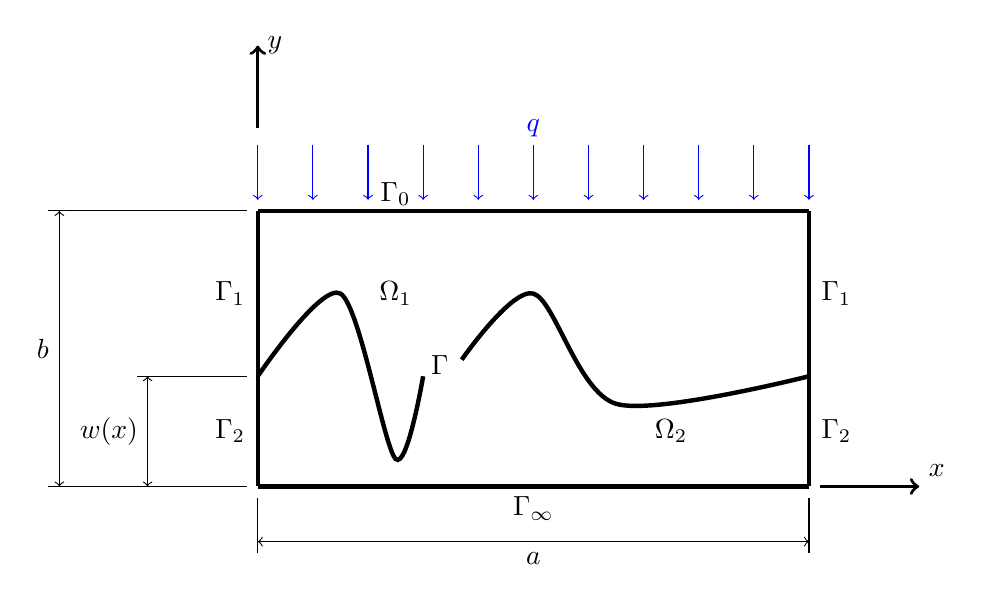
\begin{tikzpicture}[scale=0.7]

	\draw [ultra thick] (0, 0) -- (10, 0);
	%\draw [ultra thick] (0, 2) -- (7, 2);
	%\draw [ultra thick] (8, 2) -- (10, 2);
	\draw [ultra thick] plot [smooth] coordinates {(0, 2) (1.5, 3.5) (2.5, 0.5) (3, 2)};
	\draw [ultra thick] plot [smooth] coordinates {(3.7, 2.3) (5, 3.5) (6.5, 1.5) (10, 2)};
	\draw [ultra thick] (0, 5) -- (10, 5);
	\draw [ultra thick] (0, 0) -- (0, 5);
	\draw [ultra thick] (10, 0) -- (10, 5);
	
	\draw (2.5, 3.5) node {$\Omega_1$};
	\draw (7.5, 1) node {$\Omega_2$};	
	\draw (3.3, 2.2) node {$\Gamma$};
	\draw (-0.5, 3.5) node {$\Gamma_1$};
	\draw (-0.5, 1) node {$\Gamma_2$};
	\draw (10.5, 3.5) node {$\Gamma_1$};
	\draw (10.5, 1) node {$\Gamma_2$};
	\draw (5, -0.4) node {$\Gamma_\infty$};
	\draw (2.5, 5.3) node {$\Gamma_0$};
	\draw [blue](5, 6.5) node {$q$};
	\draw (5, -1.3) node {$a$};
	\draw (-3.9, 2.5) node {$b$};
	\draw (-2.7, 1) node {$w(x)$};
	
	\node [above right] at (12, 0) {$x$};
	\node [right] at (0, 8) {$y$};
	
	\draw [->, blue] (0, 6.2) -- (0, 5.2);
	\draw [->, blue] (1, 6.2) -- (1, 5.2);
	\draw [->, blue] (2, 6.2) -- (2, 5.2);
	\draw [->, blue] (3, 6.2) -- (3, 5.2);
	\draw [->, blue] (4, 6.2) -- (4, 5.2);
	\draw [->, blue] (5, 6.2) -- (5, 5.2);
	\draw [->, blue] (6, 6.2) -- (6, 5.2);
	\draw [->, blue] (7, 6.2) -- (7, 5.2);
	\draw [->, blue] (8, 6.2) -- (8, 5.2);
	\draw [->, blue] (9, 6.2) -- (9, 5.2);
	\draw [->, blue] (10, 6.2) -- (10, 5.2);
	
	\draw [->, very thick] (10.2,0) -- (12,0);
	\draw [->, very thick] (0, 6.5) -- (0,8);
	
	\draw [-] (0, -0.2) -- (0, -1.2);
	\draw [-] (10, -0.2) -- (10, -1.2);
	\draw [<->] (0, -1) -- (10, -1);
	
	\draw [-] (-0.2, 0) -- (-3.8, 0);
	\draw [-] (-0.2, 5) -- (-3.8, 5);
	\draw [-] (-0.2, 2) -- (-2.2, 2);
	\draw [<->] (-3.6, 0) -- (-3.6, 5);
	\draw [<->] (-2.0, 0) -- (-2.0, 2);

\end{tikzpicture}
\caption{Geometria do problema físico}
\label{fig2}
\end{center}
\end{figure}

Considera-se então um corpo de prova ($\Omega$) de seção transversal retangular composto por dois materiais ou regiões isotrópicas ($\Omega_1$ e $\Omega_2$), com
condutividades térmicas correspondentes $k_1$  e $k_2$, colocados em contato,
criando uma interface $\Gamma$ na qual se assume a existência de uma CTC variável com a posição $h_\Gamma(x)$.
As superfícies laterais ($\Gamma_1$ e $\Gamma_2$) das duas camadas são mantidas isoladas termicamente;
a superfície inferior ($\Gamma_\infty$) é submetida a uma temperatura prescrita; a superfície superior ($\Gamma_0$) é submetida
a um fluxo de calor por unidade de área $q$. A interseção de qualquer plano paralelo ao plano coordenado $xy$ com a interface $\Gamma$ gera uma
curva descrita por uma equação da forma $y = w(x)$.

Resumidamente, as seguintes hipóteses simplificadores foram adotadas:
\begin{itemize}
  \item O problema de condução de calor sobre o corpo de prova é em regime estacionário: $\displaystyle\frac{\partial T}{\partial t} = 0$;
  \item As condutividades térmicas $k_1$ e $k_2$ dos materiais são constantes;
  \item A variação espacial da CTC é unidimensional: $h_c \equiv h_c(x)$;
  \item O fluxo de calor $q$ sobre a superfície superior $\Gamma_0$ é constante e uniformemente distribuído;
  \item Não há dependência dos campos de temperatura com a componente $z$, ou seja, $T \equiv T(x, y)$; e
  \item Condição de contorno de terceiro tipo, ou de Robin, na interface $\Gamma$:
  		\begin{equation*}
  			-k_1\frac{\partial T_1}{\partial \mathbf{n}_1} = h_c(T_1 - T_2),
  		\end{equation*}   
\end{itemize} 
onde
$\mathbf{n}_1$ é o vetor normal à superfície $\Gamma$ e apontando para fora da região $\Omega_1$, e $T_1$ e $T_2$ são as temperaturas
correspondentes respectivamente às camadas $\Omega_1$ e $\Omega_2$, verificadas na interface $\Gamma$.

\subsection{Formulação matemática do problema direto}\label{sec_formulacao_direta}
Com base nas observações anteriores, podemos formular o problema direto de condução de calor em regime permanente através do corpo de prova $\Omega$ como segue: 

\begin{subequations}
\begin{alignat}{2}
	& \nabla^2 T_1 = 0 \quad\quad\quad\quad\quad && \text{ em } \Omega_1 \label{harm_T1} \\ \nonumber \\
	& -k_1 \frac{\partial T_1}{\partial\mathbf{n}_1} = q && \text{ em } \Gamma_0  \label{cc_T1_2} \\ \nonumber \\
	& \frac{\partial T_1}{\partial \mathbf{n}_1} = 0 && \text{ em }  \Gamma_1 \label{cc_T1_1} \\ \nonumber \\
	& -k_1 \frac{\partial T_1}{\partial\mathbf{n}_1} = h_c(T_1-T_2) \quad\quad\quad\quad\quad\quad\quad\quad && \text{ em }  \Gamma \label{cc_grad_T1} \\ \nonumber \\
	& \nabla^2 T_2 = 0 && \text{ em }  \Omega_2 \label{harm_T2} \\ \nonumber \\
	& \frac{\partial T_2}{\partial \mathbf{n}_2} = 0 && \text{ em }  \Gamma_2 \label{cc_T1_3} \\ \nonumber \\
	& T_2 = 0 && \text{ em }  \Gamma_\infty \label{cc_T1_4} \\ \nonumber \\
	& k_2\frac{\partial T_2}{\partial\mathbf{n}_2} = - k_1\frac{\partial T_1}{\partial\mathbf{n}_1} && \text{ em }  \Gamma \label{cc_T1_5}
\end{alignat}
\end{subequations}

A atribuição do valor zero à temperatura na superfície inferior $\Gamma_\infty$ do corpo $\Omega_2$, ao invés do valor prescrito, é uma simplificação
que permite a homogeinização da condição de contorno \eqref{cc_T1_4}. De fato, representando o valor da temperatura prescrita nessa superfície como $T^\star$,
o campo de temperaturas na região $\Omega_2$ seria dado por
\begin{equation}
	T_2^\star = T_2 + T^\star
\end{equation}

\newpage

\section{Problema inverso}\label{sec_prob_inv}

O problema inverso proposto neste trabalho é a estimativa da condutância térmica de contato $h_c$ na interface $\Gamma$ entre os corpos materiais
postos em contato $\Omega_1$ e $\Omega_2$, segundo o arranjo físico ilustrado na figura \ref{fig2}, conforme estabelecido na equação \eqref{eq:definicao_1}:
\begin{equation}
	h_c = \frac{q_c}{\Delta T_c}
\end{equation}

O fluxo de calor por unidade de área $q_c$ e o salto de temperatura $\Delta T_c$, ambos tomados na interface de contato, serão estimados de forma
indireta e não intrusiva, através do emprego do conceito de funcional de reciprocidade (FR), que será explicado na próxima seção.

A estimativa da CTC será feita através de medidas de temperaturas tomadas na superfície superior $\Gamma_0$ do corpo de prova, submetida a um fluxo
de calor por unidade de área $q$. As superfícies laterais $\Gamma_1$ e $\Gamma_2$ são mantidas termicamente isoladas, e a temperatura da superfície
inferior $\Gamma_\infty$ é mantida constante. As características termofísicas dos corpos materiais em contato são conhecidas, a saber, as 
condutividades térmicas $k_1$ e $k_2$, bem como as dimensões $a$ e $b$ do corpo de prova e a curva $y = w(x)$, que descreve geometricamente a interface
de contato entre os corpos. 

\subsection{Definição do conceito de funcional de reciprocidade}

A ideia do funcional de reciprocidade teve origem a partir do trabalho de \cite{artigo_andrieux}, que introduziram o conceito de funcional de descontinuidade
de reciprocidade (do inglês, \textit{reciprocity gap functional}). Segundo os autores, a intenção era levantar informações sobre a estrutura interna de
um corpo a partir de grandezas medidas na fronteira deste corpo, posto que tais grandezas estivessem relacionadas a um fenômeno físico descrito por
equações diferenciais parciais elípticas. As informações obtidas, por sua vez, seriam caracterizações de descontinuidades, espaços vazios internos ou inclusões
de materiais, entendidas de forma geral como ``perturbações''. Os autores, no referido trabalho, concentraram-se no problema específico de identificação
de falhas planas no interior de corpos materiais.

Nesse sentido, a introdução de uma perturbação a um corpo material geraria uma resposta à aplicação de um campo escalar diferente da obtida se
essa perturbação não estivesse presente. Seja então um fluxo de uma grandeza escalar $\Phi_m$ imposto à fronteira externa $\partial\Omega$ de um corpo material
$\Omega$, e seja $U_m$ a medida de um campo escalar $u$ em equilíbrio, tomada na mesma fronteira (figura \ref{fig3}). Exemplos de grandezas dessa natureza são
temperatura e fluxo de calor, ou deformação e vetor tensão. 
\begin{figure}[h!b]
\begin{center}
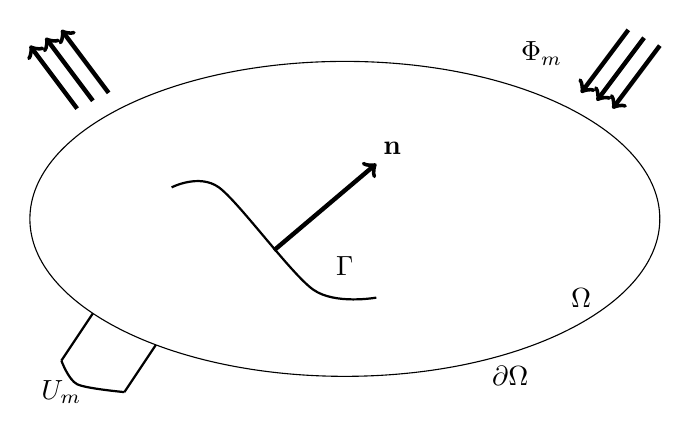
\begin{tikzpicture}[scale=1.0]
	\draw (0,0) ellipse (4cm and 2cm);
	\draw [->, ultra thick] (-3.4cm, 1.4cm) -- (-4.0cm, 2.2cm);
	\draw [->, ultra thick] (-3.2cm, 1.5cm) -- (-3.8cm, 2.3cm);
	\draw [->, ultra thick] (-3.0cm, 1.6cm) -- (-3.6cm, 2.4cm);
	\draw [->, ultra thick] (4.0cm, 2.2cm) -- (3.4cm, 1.4cm);
	\draw [->, ultra thick] (3.8cm, 2.3cm) -- (3.2cm, 1.5cm);
	\draw [->, ultra thick] (3.6cm, 2.4cm) -- (3.0cm, 1.6cm);
	\draw (2.5, 2.1) node {$\Phi_m$};
	\draw [thick] plot [smooth] coordinates {(-2.2, 0.4) (-1.6, 0.4) (-0.4, -0.9) (0.4, -1.0)};
	\draw (0.0, -0.6) node {$\Gamma$};
	\draw [->, ultra thick] (-0.9, -0.4) -- (0.4, 0.7);
	\draw (0.6, 0.9) node {$\mathbf{n}$};
	\draw (3.0, -1.0) node {$\Omega$};
	\draw (2.1, -2.0) node {$\partial\Omega$};
	\draw [thick] (-3.2cm, -1.2cm) -- (-3.6cm, -1.8cm);
	\draw [thick] (-2.4cm, -1.6cm) -- (-2.8cm, -2.2cm);
	\draw [thick] plot [smooth] coordinates {(-3.6cm, -1.8cm) (-3.4, -2.1) (-2.8cm, -2.2cm)};
	\draw (-3.6cm, -2.2cm) node {$U_m$};
\end{tikzpicture}
\caption{Corpo material $\Omega$ (adaptado de \citeauthor{artigo_andrieux}, \citeyear{artigo_andrieux})}
\label{fig3}
\end{center}
\end{figure}

A expressão que define o funcional de descontinuidade de reciprocidade, estabelecida por Andrieux e Ben Abda, é dada por:
\begin{align}
	RG(v) = \int_{\partial\Omega} \left( \Phi_m v - U_m \nabla v \cdot \mathbf{n} \right) \label{definicao_rgap}
\end{align}
onde $v$ é um outro campo potencial em equilíbrio em $\Omega$.

Os autores afirmam que quando não há descontinuidades no interior de $\Omega$, a integral \eqref{definicao_rgap} se anula. Desse modo, o funcional de descontinuidade de reciprocidade
forneceria uma medida do desvio provocado num campo escalar $u$ no corpo $\Omega$ submetido a um fluxo $\Phi_m$ em sua superfície, se esse corpo
possuir uma descontinuidade $\Gamma$ em seu interior.

É importante destacar que a integral \eqref{definicao_rgap} é calculada sobre o contorno da fronteira do corpo material $\Omega$, onde as grandezas envolvidas devem
ser efetivamente conhecidas. Assim, é possível inferir características no interior do corpo a partir de medições tomadas em seu contorno.

\subsection{Aplicação do funcional de reciprocidade na dedução da expressão da estimativa da condutância térmica de contato}\label{secao_sobre_fr}

Baseados no conceito de funcional de descontinuidade de reciprocidade, \cite{reciproc_2} apresentaram um trabalho pioneiro em que estabeleceram uma
técnica não intrusiva e não iterativa para solução de problemas inversos de transferência de calor, voltada para a estimativa da resistência térmica de
contato (RTC) entre dois corpos. A metodologia aplicada nesta dissertação, baseada no referido trabalho e em trabalhos posteriores em que aquele conceito
foi utilizado \citep{artigo_padilha_3}, será descrita nos parágrafos a seguir. 

\cite{reciproc_2} adaptaram o termo original definido em \eqref{definicao_rgap} para o problema formulado na seção \ref{sec_formulacao_direta},
introduzindo o conceito de funcional de reciprocidade (FR) através da seguinte expressão:
\begin{align}
	\Re(F) = \int_{\Gamma_0}\left[\left(\frac{-q}{k_1}\right)F - Y\frac{\partial F}{\partial\mathbf{n_1}}\right]d\Gamma_0
	\label{def_funcional_reciprocidade}
\end{align}
onde $F$ é uma função associada a um campo potencial auxiliar em equilíbrio em $\Omega_1$, $k_1$ é a condutividade térmica do material $\Omega_1$, $q$ é o fluxo de calor por unidade de área
aplicado na superfície externa $\Gamma_0$ e $Y$ são medidas de temperatura tomadas na mesma superfície $\Gamma_0$. O vetor $\mathbf{n_1}$ é o vetor normal à superfície
$\Gamma_0$ e apontando para fora do contorno do material $\Omega_1$.

De forma análoga à equação \eqref{definicao_rgap}, a equação \eqref{def_funcional_reciprocidade} permite medir a alteração do campo de temperatura
gerado por um fluxo de calor por unidade de área $q$ aplicado na superfície externa $\Gamma_0$ do material compósito $\Omega$ devido à existência
de uma descontinuidade $\Gamma$ em seu interior; essa alteração está relacionada à existência de uma RTC nessa interface. No caso de não haver descontinuidade
em $\Omega$, a integral \eqref{def_funcional_reciprocidade} se anula.

Em seu trabalho, \cite{reciproc_2} formulam dois problemas difusivos para determinação de duas classes de funções auxiliares $F_1$ e $G_1$, no mesmo domínio físico da região compreendida
por $\Omega_1$. Os problemas formulados são análogos ao problema de difusão de temperatura formulado em \eqref{harm_T1}--\eqref{cc_T1_5}, porém empregando condições de contorno apropriadas, que
serão detalhadas na seção \ref{secao_probs_aux}.

Através dessas condições de contorno, os autores demonstram as seguintes identidades:
\begin{align}
	k_1 \int_{\Gamma_0}\left[\left(\frac{-q}{k_1}\right)F_1 - Y\frac{\partial F_1}{\partial\mathbf{n_1}}\right]d\Gamma_0
	=
	\int_\Gamma k_1 \frac{\partial F_1}{\partial\mathbf{n_1}}\left(T_1 - T_2\right)d\Gamma
	\label{identidade_T}
\end{align}
\begin{align}
	k_1 \int_{\Gamma_0}\left[\left(\frac{-q}{k_1}\right)G_1 - Y\frac{\partial G_1}{\partial\mathbf{n_1}}\right]d\Gamma_0
	=
	\int_\Gamma -k_1 G_1 \frac{\partial T_1}{\partial\mathbf{n_1}}d\Gamma
	\label{identidade_q}
\end{align}

Os termos à esquerda das equações \eqref{identidade_T} e \eqref{identidade_q} são, a menos da constante multiplicativa $k_1$, a definição do funcional de reciprocidade para as 
funções auxiliares $F_1$ e $G_1$.

As integrais à direita têm um significado importante. É possível observar que elas são calculadas \textit{ao longo da interface de contato} $\Gamma$. O termo
$T_1 - T_2$ é exatamente \textit{o salto de temperatura através da interface} $\Gamma$, enquanto que o termo $\displaystyle-k_1 \frac{\partial T_1}{\partial\mathbf{n_1}}$
é exatamente \textit{o fluxo de calor por unidade de área através da interface} $\Gamma$ (cf. equação \eqref{eq:definicao_2}). Desse modo, as identidades \eqref{identidade_T} e \eqref{identidade_q}
relacionam \textit{as medidas
do salto de temperatura e de fluxo de calor na interface} $\Gamma$ -- grandezas cuja razão fornece a RTC sobre a interface -- com \textit{as medidas de temperatura} $Y$ \textit{tomadas na superfície} $\Gamma_0$.

Estas mesmas integrais também podem ser interpretadas à luz dos conceitos de Álgebra Linear \citep{livro_axler}. Sob esse ponto de vista, os termos
$\displaystyle k_1 \frac{\partial F}{\partial\mathbf{n_1}}$, $T_1 - T_2$, $G$ e $\displaystyle-k_1 \frac{\partial T_1}{\partial\mathbf{n_1}}$ podem ser identificados como funções pertencentes a um espaço
linear de funções, denotado por $L^2(\Gamma)$, em que se define a operação de produto interno como segue:
\begin{align}
	\langle f_1, f_2\rangle_{L^2(\Gamma)} = \int_\Gamma f_1(\Gamma) f_2(\Gamma) d\Gamma \label{definicao_innner_product}
\end{align} 
onde $f_1$ e $f_2$ são funções reais, contínuas por partes, definidas a longo do contorno $\Gamma$ sobre o qual é calculada a integral. A norma de uma
função, que é uma métrica análoga ao ``comprimento'' ou ``distância'', é definida nesse espaço linear como\footnote{A partir desse ponto, o subscrito ${L^2(\Gamma)}$ será
subentendido nas transcrições de produtos internos, para fins de simplificação gráfica das equações.}:
\begin{align}
	\norm{f} = \sqrt{\langle f, f\rangle}
\end{align}

A partir de parametrizações convenientes dos problemas difusivos auxiliares, é possível levantar duas famílias de funções auxiliares $F_{1,j}, j=1,2,\ldots N_1$
e $G_{1,j}, j=1,2,\ldots N_2$. Assim, através da definição de produto interno em \eqref{definicao_innner_product} e da definição de funcional de reciprocidade em \eqref{def_funcional_reciprocidade},
as identidades \eqref{identidade_T} e \eqref{identidade_q} podem ser reescritas como:
\begin{align}
	k_1 \Re(F_{1,j})
	=
	\left\langle \left[T_1 - T_2\right]_\Gamma, \beta_j\right\rangle
	\label{identidade_T_inner}
\end{align}
\begin{align}
	k_1 \Re(G_{1,j})
	=
	\left\langle  -k_1 \frac{\partial T_1}{\partial\mathbf{n_1}}\bigg|_\Gamma, \gamma_j\right\rangle
	\label{identidade_q_inner}
\end{align}
onde
\begin{align}
	\beta_j = k_1 \frac{\partial F_{1,j}}{\partial\mathbf{n_1}}\bigg|_\Gamma \label{expressao_define_beta}
\end{align}
\begin{align}
	\gamma_j = G_{1,j}\big|_\Gamma \label{expressao_define_gamma}
\end{align}

Com base no trabalho de \cite{artigo_padilha_3}, será proposta uma escolha de parametrização de condições de contorno dos problemas auxiliares de modo que as funções
$\beta_j, j=1,2,\ldots N_1$ e $\gamma_j, j=1,2,\ldots N_2$ formem dois conjuntos ortonormais, isto é:
\begin{align}
	\left\langle  \beta_m, \beta_n \right\rangle = \left\lbrace
		\begin{matrix}
		0, & m \neq n \\
		1, & m = n 
		\end{matrix}
	\right.
\end{align}
\begin{align}
	\left\langle  \gamma_m, \gamma_n \right\rangle = \left\lbrace
		\begin{matrix}
		0, & m \neq n \\
		1, & m = n 
		\end{matrix}
	\right.
\end{align}

Nessas condições, cada um dos conjuntos define um subespaço linear contido no espaço linear $L^2(\Gamma)$. Os subespaços lineares gerados pela bases
ortonormais $\beta_j$ e $\gamma_j$ serão denotados respectivamente por $L^2(\Gamma, \beta)$ e $L^2(\Gamma, \gamma)$.

Por definição, a \textit{projeção ortogonal} de uma função $f$ pertencente ao espaço linear $L^2(\Gamma)$ sobre o subespaço linear $L^2(\Gamma, \epsilon)$
gerado por uma base ortonormal $\epsilon_j, j=1,2,\ldots,N$ é dada por:
\begin{align}
	P_{L^2(\Gamma, \epsilon)}[f] = \sum_{j=1}^N \left\langle f, \epsilon_j \right\rangle \epsilon_j
\end{align}

A projeção ortogonal provê uma forma aproximada de se representar uma função $f$ como combinação linear dos elementos de uma base ortonormal de
funções. Com efeito, seja $g$ uma função em $L^2(\Gamma, \epsilon)$, e que portanto pode ser expandida como uma combinação linear dos elementos da base $\epsilon_j$. Uma métrica de
avaliação da ``distância'' entre as funções $f$ e $g$ é dada pela norma da diferença entre essas funções. O menor valor possível para essa norma ocorre
quando a função $g$ for a projeção ortogonal de $f$ sobre $L^2(\Gamma, \epsilon)$ \citep{livro_axler}. Ou seja,
\begin{align}
	\norm{f - P_{L^2(\Gamma, \epsilon)}[f]} \le \norm{f - g}, \forall g \in L^2(\Gamma, \epsilon)
\end{align}

Dessa forma, o salto de temperatura e o fluxo de calor por unidade de área na interface $\Gamma$ podem ser representados de forma aproximada através de projeções
ortogonais sobre os subespaços lineares $L^2(\Gamma, \beta)$ e $L^2(\Gamma, \gamma)$ respectivamente:
\begin{align}
[T_1 - T_2]_\Gamma \approx \sum_{j=1}^{N_1} \left\langle  \left[T_1 - T_2\right]_\Gamma, \beta_j \right\rangle \beta_j
\end{align}
\begin{align}
	- k_1 \frac{\partial T_1}{\partial\mathbf{n_1}}\bigg|_\Gamma \approx \sum_{j=1}^{N_2} \left\langle  -k_1 \frac{\partial T_1}{\partial\mathbf{n_1}}\bigg|_\Gamma, \gamma_j \right\rangle \gamma_j
\end{align}

Aplicando as identidades \eqref{identidade_T_inner} e \eqref{identidade_q_inner} às equações acima, e assumindo que as projeções ortogonais representam
de forma razoável as funções correspondentes, pode-se escrever:
\begin{align}
	[T_1 - T_2]_\Gamma = \sum_{j=1}^{N_1} k_1 \Re(F_{1,j}) \beta_j \label{resultado_1}
\end{align}
\begin{align}
	- k_1 \frac{\partial T_1}{\partial\mathbf{n_1}}\bigg|_\Gamma = \sum_{j=1}^{N_2} k_1 \Re(G_{1,j}) \gamma_j \label{resultado_2}
\end{align}

Finalmente, substituindo os resultados obtidos em \eqref{resultado_1} e \eqref{resultado_2} na definição de condutância térmica de contato,
\eqref{eq:definicao_3}, obtemos a seguinte relação:
\begin{align}
	& h_c % = \frac{- k_1 \displaystyle\frac{\partial T_1}{\partial\mathbf{n_1}}\bigg|_\Gamma}{[T_1 - T_2]_\Gamma} 
	= \frac{\displaystyle\sum_{j=1}^{N_2} \Re(G_{1,j}) \gamma_j}{\displaystyle\sum_{j=1}^{N_1} \Re(F_{1,j}) \beta_j}
	\label{equacao_definicao_f_r}
\end{align}
ou, de forma mais explícita:
\begin{align}
	& h_c % = \frac{- k_1 \displaystyle\frac{\partial T_1}{\partial\mathbf{n_1}}\bigg|_\Gamma}{[T_1 - T_2]_\Gamma} 
	= \frac{\displaystyle\sum_{j=1}^{N_2} \gamma_j\int_{\Gamma_0}\left[\left(\frac{-q}{k_1}\right)G_{1,j} - Y\frac{\partial G_{1,j}}{\partial\mathbf{n_1}}\right]d\Gamma_0}{\displaystyle\sum_{j=1}^{N_1} \beta_j \int_{\Gamma_0}\left[\left(\frac{-q}{k_1}\right)F_{1,j} - Y\frac{\partial F_{1,j}}{\partial\mathbf{n_1}}\right]d\Gamma_0}
	\label{equacao_definicao_f_r_expl}
\end{align}

A expressão \eqref{equacao_definicao_f_r} permite calcular a estimativa da distribuição da CTC ao longo da interface de contato $\Gamma$, conhecendo-se
a distribuição de temperaturas $Y$ medidas na face externa superior do arranjo físico da figura \ref{fig2}, eliminando assim a necessidade prévia de
se conhecer informações e características internas do corpo de prova, tais como rugosidade entre as superfícies em contato, pressão de contato, ou
o fluido presente no interstício. As determinações do salto de temperatura e fluxo de calor por unidade de área na interface de contato são feitas de forma indireta, através
das expansões em funções ortonormais expressas em \eqref{resultado_1} e \eqref{resultado_2}, o que indica o caráter não intrusivo da técnica.

Quanto ao aspecto numérico-computacional, é possível notar que as integrais que fornecem os funcionais de reciprocidade só precisam ser calculadas
uma única vez, para uma determinada caracterização geométrica e termofísica do problema. As classes de funções $F_{1,j}$ e $G_{1,j}$, obtidas através da resolução dos
problemas difusivos auxiliares, dependem unicamente das
características geométricas (comprimento e largura do corpo de prova, e a curva $y = w(x)$ que descreve o formato da interface)
e termofísicas (condutâncias térmicas $k_1$ e $k_2$ dos materiais em contato). Por essa razão, o método é classificado como não iterativo, visto que
a obtenção da estimativa da CTC em algum ponto sobre a interface se resume à substituição dos valores de $\beta_j$ e $\gamma_j$ avaliados naquele
ponto nos somatórios da equação \eqref{equacao_definicao_f_r}.

Por último, é importante destacar que a expressão \eqref{equacao_definicao_f_r} permite a estimativa da CTC para qualquer formato de interface $\Gamma$,
desde que se conheça a sua descrição analítica representada pela curva $y = w(x)$. O caso particular em que a interface é plana e paralela às bases do corpo
de prova foi resolvido analiticamente por \cite{tese_padilha}.

% \subsection{Comentários sobre o caso particular de interface de contato plana}
% 
% O problema inverso definido pelo arranjo físico representado na figura \ref{fig2}, juntamente com as equações \eqref{harm_T1} -- \eqref{cc_T1_5}, é uma
% generalização de um problema mais simples em que a interface de contato é um plano paralelo às faces inferior e superior do corpo de prova, conforme
% ilustrado na \ref{fig4}.
\begin{figure}[h!b]
\begin{center}
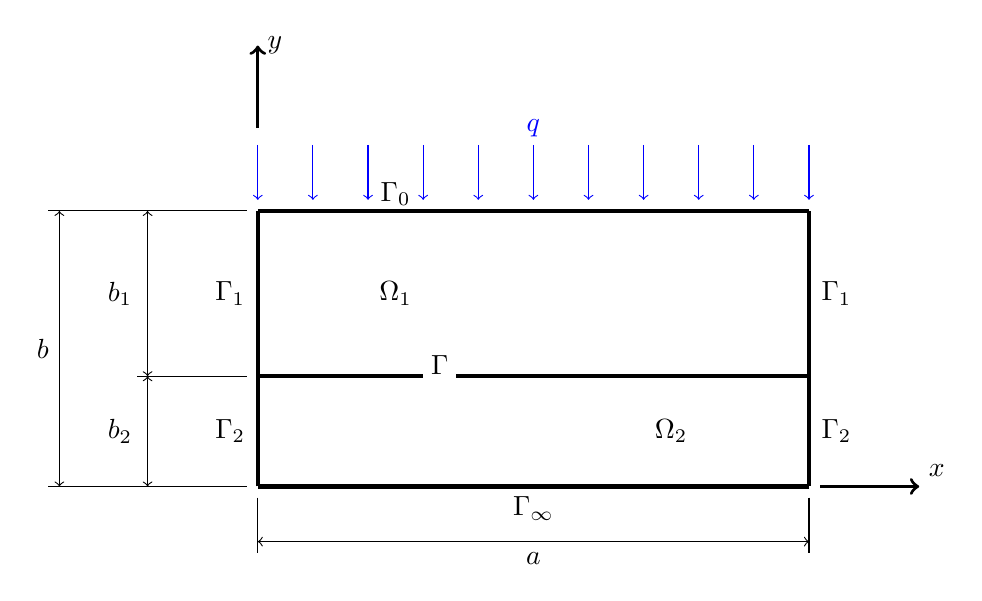
\begin{tikzpicture}[scale=0.7]

	\draw [ultra thick] (0, 0) -- (10, 0);
	%\draw [ultra thick] (0, 2) -- (7, 2);
	%\draw [ultra thick] (8, 2) -- (10, 2);
	\draw [ultra thick] (0, 5) -- (10, 5);
	\draw [ultra thick] (0, 2.0) -- (3.0, 2.0);
	\draw [ultra thick] (3.6, 2.0) -- (10, 2.0);
	\draw [ultra thick] (0, 0) -- (0, 5);
	\draw [ultra thick] (10, 0) -- (10, 5);

	\draw (2.5, 3.5) node {$\Omega_1$};
	\draw (7.5, 1) node {$\Omega_2$};
	\draw (3.3, 2.2) node {$\Gamma$};
	\draw (-0.5, 3.5) node {$\Gamma_1$};
	\draw (-0.5, 1) node {$\Gamma_2$};
	\draw (10.5, 3.5) node {$\Gamma_1$};
	\draw (10.5, 1) node {$\Gamma_2$};
	\draw (5, -0.4) node {$\Gamma_\infty$};
	\draw (2.5, 5.3) node {$\Gamma_0$};
	\draw [blue](5, 6.5) node {$q$};
	\draw (5, -1.3) node {$a$};
	\draw (-3.9, 2.5) node {$b$};
	\draw (-2.5, 1) node {$b_2$};
	\draw (-2.5, 3.5) node {$b_1$};

	\node [above right] at (12, 0) {$x$};
	\node [right] at (0, 8) {$y$};

	\draw [->, blue] (0, 6.2) -- (0, 5.2);
	\draw [->, blue] (1, 6.2) -- (1, 5.2);
	\draw [->, blue] (2, 6.2) -- (2, 5.2);
	\draw [->, blue] (3, 6.2) -- (3, 5.2);
	\draw [->, blue] (4, 6.2) -- (4, 5.2);
	\draw [->, blue] (5, 6.2) -- (5, 5.2);
	\draw [->, blue] (6, 6.2) -- (6, 5.2);
	\draw [->, blue] (7, 6.2) -- (7, 5.2);
	\draw [->, blue] (8, 6.2) -- (8, 5.2);
	\draw [->, blue] (9, 6.2) -- (9, 5.2);
	\draw [->, blue] (10, 6.2) -- (10, 5.2);

	\draw [->, very thick] (10.2,0) -- (12,0);
	\draw [->, very thick] (0, 6.5) -- (0,8);

	\draw [-] (0, -0.2) -- (0, -1.2);
	\draw [-] (10, -0.2) -- (10, -1.2);
	\draw [<->] (0, -1) -- (10, -1);

	\draw [-] (-0.2, 0) -- (-3.8, 0);
	\draw [-] (-0.2, 5) -- (-3.8, 5);
	\draw [-] (-0.2, 2) -- (-2.2, 2);
	\draw [<->] (-3.6, 0) -- (-3.6, 5);
	\draw [<->] (-2.0, 0) -- (-2.0, 2);
	\draw [<->] (-2.0, 2) -- (-2.0, 5);

\end{tikzpicture}
\caption{Geometria do problema físico resolvido por \cite{reciproc_2}}
\label{fig4}
\end{center}
\end{figure}
% 
% Na resolução deste problema inverso, \cite{reciproc_2} deduziram uma versão mais simples da expressão \eqref{equacao_definicao_f_r}:
% \begin{align}
% 	& h_c % = \frac{- k_1 \displaystyle\frac{\partial T_1}{\partial\mathbf{n_1}}\bigg|_\Gamma}{[T_1 - T_2]_\Gamma} 
% 	= \frac{\displaystyle\sum_{j=1}^N \Re(G_{1,j}) \phi_j}{\displaystyle\sum_{j=1}^N \Re(F_{1,j}) \phi_j}
% 	\label{equacao_definicao_f_r_simples}
% \end{align}
% 
% As funções $\phi_j, j=1,2\ldots,N$ foram definidas através de funções seno e cosseno, ortogonais
% no intervalo $0 \le x \le a$.
% 
% Uma vez que, para esse problema, $\phi_j = \beta_j = \gamma_j$, foram definidas as seguintes condições de contorno para as famílias de 
% funções $F_{1,j}$ e $G_{1,j}$: 
% 
% 
%  
% . Os problemas difusivos auxiliares que fornecem as funções $F_j$ e $G_j$
% foram resolvidos através do Método das Soluções Fundamentais 

\include{03_resolucao}
\section{Formulação analítica para a condutância térmica de contato}

Nas últimas seções, foram finalmente deduzidas as expressões para as funções auxiliares $F_{1,j}$ e $G_{1,j}$, bem como as funções $\beta_j$ e $\gamma_j$ que compõem as bases ortonormais em $L^2(\Gamma)$. Nesta seção, estes resultados serão reunidos, a fim de levantar uma expressão analítica de uso geral, para estimativa da condutância térmica de contato ao longo da superfície irregular $\Gamma$. Como ponto de partida, será estabelecida a expressão em coordenadas cartesianas do produto interno entre as funções no espaço linear $L^2(\Gamma)$.

\subsection{Formulação do produto interno no espaço linear de funções $L^2(\Gamma)$ em coordenadas cartesianas}

Na seção \ref{secao_sobre_fr}, foi definido na equação \eqref{definicao_innner_product} o produto interno entre duas funções $f_1$ e $f_2$ no espaço linear de funções $L^2(\Gamma)$:
\begin{align}
\langle f_1, f_2\rangle = \int_\Gamma f_1(\Gamma) f_2(\Gamma) d\Gamma \label{integral_da_definicao_produto_interno}
\end{align}

Se a superfície $\Gamma$, sobre a qual é realizada a integração, possuir uma representação paramétrica da forma
\begin{align}
\mathbf{\Gamma}(t) = x(t)\mathbf{a}_x + y(t)\mathbf{a}_y
\end{align}
onde $\mathbf{a}_x$ e $\mathbf{a}_y$ são os vetores unitários da base canônica do sistema cartesiano, então a integral \eqref{integral_da_definicao_produto_interno} pode ser escrita como \citep{livro_stewart}:
\begin{align}
\langle f_1, f_2\rangle = \int_{t=t_0}^{t=t_1}f_1(x(t), y(t))f_2(x(t), y(t))\sqrt{x'(t)^2 + y'(t)^2}dt \label{integral_da_definicao_produto_interno_2}
\end{align}

Adotando as parametrizações \eqref{parametrizacao_x} e \eqref{parametrizacao_y}, pode-se escrever:
\begin{align} 
\langle f_1, f_2\rangle = \int_{t=0}^{t=a}f_1(t, w(t))f_2(t, w(t))\sqrt{1 + w'(t)^2}dt \label{integral_da_definicao_produto_interno_3}
\end{align}
ou, uma vez que $x$ e $t$ são equivalentes,
\begin{align}
\langle f_1, f_2\rangle = \int_{x=0}^{x=a}f_1(x, w(x))f_2(x, w(x))\sqrt{1 + w'(x)^2}dx \label{integral_da_definicao_produto_interno_4}
\end{align}

\subsection{Formulação da estimativa da condutância térmica de contato em coordenadas cartesianas}

Os funcionais de reciprocidade, conforme dito na seção \ref{secao_sobre_fr}, são ferramentas através das quais será estimada a condutância térmica de contato (CTC) na interface de contato $\Gamma$. A expressão \eqref{def_funcional_reciprocidade} fornece o funcional de reciprocidade para uma função $F(x, y)$:
\begin{align}
\Re(F)
=
\int_{\Gamma_0}\left[\left(\frac{-q}{k_1}\right)F - Y\frac{\partial F}{\partial\mathbf{n_1}}\right]d\Gamma_0
\label{integral_de_contorno_para_F}
\end{align}

A superfície $\Gamma_0$, representada no arranjo da figura \ref{fig2}, e sobre a qual é calculada a integral de contorno \eqref{integral_de_contorno_para_F}, pode ser parametrizada como:
\begin{align}
\mathbf{\Gamma}_0(t) = t\mathbf{a}_x + b \mathbf{a}_y
\end{align}
onde $b$ é o comprimento vertical do corpo de prova representado na figura \ref{fig2}.

O vetor $\mathbf{n}_1$, normal à superfície $\Gamma_0$, é o próprio vetor unitário $\mathbf{a}_y$ da base canônica. Logo, a derivada direcional de $F$ sobre esse vetor será dada por \citep{livro_stewart}:
\begin{align}
\frac{\partial F}{\partial\mathbf{n}_1}\bigg|_{\Gamma_0} & = \nabla F \cdot \mathbf{a}_y \nonumber \\
& = \left[\frac{\partial F(x, b)}{\partial x}\mathbf{a}_x + \frac{\partial F(x, b)}{\partial y}\mathbf{a}_y \right] \cdot \mathbf{a}_y \nonumber \\
& = \frac{\partial F(x, b)}{\partial y}
\end{align} 

Substituindo na integral \eqref{integral_de_contorno_para_F}, obtém-se \citep{livro_stewart}:
\begin{align}
\Re(F)
=
\int_{t=0}^{t=a} \left[\left(\frac{-q}{k_1}\right)F(t, b) - Y(t)\frac{\partial F(t, b)}{\partial y}\right] dt
\label{integral_de_contorno_para_F_2}
\end{align}
ou
\begin{align}
\Re(F)
=
\int_{x=0}^{x=a} \left[\left(\frac{-q}{k_1}\right)F(x, b) - Y(x)\frac{\partial F(x, b)}{\partial y}\right] dx
\label{integral_de_contorno_para_F_3}
\end{align}

Dessa forma, aplicando a equação \eqref{integral_de_contorno_para_F_3} para expressar os funcionais de reciprocidade das funções $F_{1,j}$ e $G_{1,j}$:
\begin{align}
\Re(F_{1,j})
=
\int_{x=0}^{x=a} \left[\left(\frac{-q}{k_1}\right)F_{1,j}(x, b) - Y(x)\frac{\partial F_{1,j}(x, b)}{\partial y}\right] dx
\label{integral_de_contorno_para_F1_0}
\end{align}
\begin{align}
\Re(G_{1,j})
=
\int_{x=0}^{x=a} \left[\left(\frac{-q}{k_1}\right)G_{1,j}(x, b) - Y(x)\frac{\partial G_{1,j}(x, b)}{\partial y}\right] dx
\label{integral_de_contorno_para_G1_0}
\end{align}
ou, substituindo as condições de contorno \eqref{funcao_F_cc_T1_2_cart} e \eqref{funcao_G_cc_T1_2_cart}:
\begin{align}
\Re(F_{1,j})
& =
\int_0^a \left[\left(\frac{-q}{k_1}\right)\psi_j(x) - Y(x)\frac{\partial F_{1,j}(x, b)}{\partial y}\right] dx \nonumber \\
& =
-\frac{q}{k_1}\int_0^a\psi_j(x)dx - \int_0^a Y(x)\frac{\partial F_{1,j}(x, b)}{\partial y} dx \nonumber \\
& =
-\frac{q}{k_1}\bar{\psi}_{j,0} - \int_0^a Y(x)\frac{\partial F_{1,j}(x, b)}{\partial y} dx
\label{integral_de_contorno_para_F1}
\end{align}
%
\begin{align}
\Re(G_{1,j})
& =
\int_0^a \left[\left(\frac{-q}{k_1}\right)\phi_j(x) - Y(x)\frac{\partial G_{1,j}(x, b)}{\partial y}\right] dx \nonumber \\
& =
-\frac{q}{k_1}\int_0^a\phi_j(x)dx - \int_0^a Y(x)\frac{\partial G_{1,j}(x, b)}{\partial y} dx
\nonumber \\
& =
-\frac{q}{k_1}\bar{\phi}_{j,0} - \int_0^a Y(x)\frac{\partial G_{1,j}(x, b)}{\partial y} dx
\label{integral_de_contorno_para_G1}
\end{align}

As derivadas em relação a $y$ de $F_{1,j}$ e $G_{1,j}$, avaliadas em $y = b$, podem ser determinadas por derivação parcial das expressões \eqref{solucao_transf_inversa_F1_com_dependencia} e
\eqref{solucao_transf_inversa_G1_com_dependencia}, truncadas até o índice $M$, fornecendo:
%
\begin{align}
\frac{\partial F_{1, j}(x, b)}{\partial y} = & \frac{\bar{\psi}_{j,0} - \mathbb{A}_{j,0}}{ab} - 
\frac{2}{a}\sum_{m=1}^M \mu_m \left(\mathbb{A}_{j,m}\frac{1}{\sinh\mu_m b} - \bar{\psi}_{j, m}\frac{\cosh\mu_m b}{\sinh\mu_m b}\right)\cos\mu_m x \nonumber \\
= & \frac{\bar{\psi}_{j,0} - \mathbb{A}_{j,0}}{ab} - 
\frac{2}{a}\sum_{m=1}^M \mu_m \left(\frac{\mathbb{A}_{j,m}}{\sinh\mu_m b} - \frac{\bar{\psi}_{j, m}}{\tanh\mu_m b}\right)\cos\mu_m x
\label{derivada_parcial_y_F}
\end{align}
%
\begin{align}
\frac{\partial G_{1, j}(x, b)}{\partial y} = & \frac{\bar{\phi}_{j,0} - \mathbb{E}_{j,0}}{ab} - 
\frac{2}{a}\sum_{m=1}^M \mu_m \left(\mathbb{E}_{j,m}\frac{1}{\sinh\mu_m b} - \bar{\phi}_{j, m}\frac{\cosh\mu_m b}{\sinh\mu_m b}\right)\cos\mu_m x \nonumber \\
= & \frac{\bar{\phi}_{j,0} - \mathbb{E}_{j,0}}{ab} - 
\frac{2}{a}\sum_{m=1}^M \mu_m \left(\frac{\mathbb{E}_{j,m}}{\sinh\mu_m b} - \frac{\bar{\phi}_{j, m}}{\tanh\mu_m b}\right)\cos\mu_m x
\label{derivada_parcial_y_G}
\end{align}

Substituindo os resultados \eqref{derivada_parcial_y_F} e \eqref{derivada_parcial_y_G} em \eqref{integral_de_contorno_para_F1} e \eqref{integral_de_contorno_para_G1}, obtém-se:
\begin{align}
\Re(F_{1,j})
& =
-\frac{q}{k_1}\bar{\psi}_{j,0} + \frac{\mathbb{A}_{j,0} - \bar{\psi}_{j,0}}{ab}\int_0^a Y(x)dx + \nonumber \\
& \frac{2}{a}\sum_{m=1}^M \mu_m \left(\frac{\mathbb{A}_{j,m}}{\sinh\mu_m b} - \frac{\bar{\psi}_{j, m}}{\tanh\mu_m b}\right)\int_0^a Y(x)\cos\mu_m x dx
\label{calculo_FR_F1_antes}
\end{align}
%
\begin{align}
\Re(G_{1,j})
& =
-\frac{q}{k_1}\bar{\phi}_{j,0} + \frac{\mathbb{E}_{j,0} - \bar{\phi}_{j,0}}{ab}\int_0^a Y(x)dx + \nonumber \\
& \frac{2}{a}\sum_{m=1}^M \mu_m \left(\frac{\mathbb{E}_{j,m}}{\sinh\mu_m b} - \frac{\bar{\phi}_{j, m}}{\tanh\mu_m b}\right)\int_0^a Y(x)\cos\mu_m x dx
\label{calculo_FR_G1_antes}
\end{align}

As equações \eqref{calculo_FR_F1_antes} e \eqref{calculo_FR_G1_antes} fornecem os funcionais de reciprocidade $\Re(F_{1,j})$ e $\Re(G_{1,j})$ referentes à uma escolha particular de funções auxiliares $\psi_j(x)$ e $\phi_j(x)$, respectivamente. Os termos $\bar{\psi}_{j, m}$ e $\bar{\phi}_{j, m}$, por sua vez, correspondem respectivamente às transformadas integrais das referidas funções $\psi_j(x)$ e $\phi_j(x)$. É necessário agora estabelecer uma escolha para estas funções que seja vantajosa do ponto de vista computacional. \cite{tese_padilha} empregou, para o caso da interface plana horizontal, as seguintes alternativas para $\psi_j(x)$ e $\phi_j(x)$:
\begin{align}
\psi_j(x), \phi_j(x) = \left\lbrace
\begin{array}{ll}
\displaystyle\sqrt{\frac{1}{a}}, & j = 0 \\ \nonumber \\
\displaystyle\sqrt{\frac{2}{a}}\cos \mu_j x, & j = 1,2,3,\ldots
\end{array}
\right.
\end{align}

As equações acima, a menos das constantes multiplicativas, são equivalentes às autofunções soluções do problema de Sturm-Liouville formulado em \eqref{problema_vc_1a}, \eqref{problema_vc_1b} e \eqref{problema_vc_1c}. Esta característica permite simplificar consideravelmente as expressões \eqref{calculo_FR_F1_antes} e \eqref{calculo_FR_G1_antes}, através da aplicação da propriedade da ortogonalidade formulada em \eqref{ortogon}. Com efeito, seja o cálculo de $\bar{\psi}_{j, m}$ através da definição da transformada integral:
\begin{align}
\bar{\psi}_{j, m} = \int_0^a \psi_j(x) X(\mu_m, x)dx \label{integrando_m}
\end{align}
onde $X(\mu_m, x)$ é definida em \eqref{definicao_das_autofuncoes}

Para o caso $j \ne 0$, pode-se escrever:
\begin{align}
\psi_j(x) = \sqrt{\frac{2}{a}}X(\mu_j, x) \label{nova_expressao_m}
\end{align}

Substituindo \eqref{nova_expressao_m} em \eqref{integrando_m}:
\begin{align}
\bar{\psi}_{j, m} & = \int_0^a \sqrt{\frac{2}{a}}X(\mu_j, x) X(\mu_m, x)dx  \nonumber \\
& = \sqrt{\frac{2}{a}} \int_0^a X(\mu_j, x) X(\mu_m, x)dx \label{integrando_m2}
\end{align}

Devido à propriedade da ortogonalidade \eqref{ortogon}, a integral em \eqref{integrando_m2} será não-nula apenas para $m = j$, e a equação \eqref{integrando_m2} pode ser escrita como:
\begin{align}
\bar{\psi}_{j, j} & = \sqrt{\frac{2}{a}} N(\mu_j) \nonumber \\
& = \sqrt{\frac{a}{2}} \label{integrando_m3}
\end{align}
sendo que foi usado o resultado em \eqref{valor_integral_norm} na simplificação da equação acima.

Para o caso $j = 0$, pode-se escrever:
\begin{align}
\psi_0(x) = \sqrt{\frac{1}{a}}X(\mu_0, x) \label{nova_expressao_0}
\end{align}

Substituindo \eqref{nova_expressao_0} em \eqref{integrando_m}:
\begin{align}
\bar{\psi}_{0, m} & = \int_0^a \sqrt{\frac{1}{a}}X(\mu_0, x) X(\mu_m, x)dx  \nonumber \\
& = \sqrt{\frac{1}{a}} \int_0^a X(\mu_0, x) X(\mu_m, x)dx \label{integrando_m0}
\end{align}

Devido à propriedade da ortogonalidade \eqref{ortogon}, a integral em \eqref{integrando_m0} será não-nula apenas para $m = 0$, e a equação \eqref{integrando_m0} pode ser escrita como:
\begin{align}
\bar{\psi}_{0, 0} & = \sqrt{\frac{1}{a}} N(\mu_0) \nonumber \\
& = \sqrt{a} \label{integrando_m00}
\end{align}
sendo que foi usado o resultado em \eqref{valor_integral_norm} na simplificação da equação acima.

Para empregar os reultados obtidos em \eqref{integrando_m3} e \eqref{integrando_m00}, será feita uma reorganização dos termos na equação \eqref{calculo_FR_F1_antes}, obtendo-se:
\begin{align}
\Re(F_{1,j})
& =
-\bar{\psi}_{j,0}\left(\frac{q}{k_1} + \frac{1}{ab}\int_0^a Y(x)dx\right) -
\frac{2}{a}\sum_{m=1}^M \mu_m \frac{\bar{\psi}_{j, m}}{\tanh\mu_m b}\int_0^a Y(x)\cos\mu_m x dx + \nonumber \\
& \frac{\mathbb{A}_{j,0}}{ab}\int_0^a Y(x)dx + \frac{2}{a}\sum_{m=1}^M \mu_m \frac{\mathbb{A}_{j,m}}{\sinh\mu_m b}\int_0^a Y(x)\cos\mu_m x dx
\end{align}
ou
\begin{align}
\Re(F_{1,j})
=
\zeta_j
+
\frac{\mathbb{A}_{j,0}}{ab}\int_0^a Y(x)dx + \frac{2}{a}\sum_{m=1}^M \mu_m \frac{\mathbb{A}_{j,m}}{\sinh\mu_m b}\int_0^a Y(x)\cos\mu_m x dx
\label{calculo_FR_F1}
\end{align}
onde
\begin{align}
\zeta_j = \left\lbrace
\begin{array}{ll}
-\sqrt{a}\displaystyle\left(\frac{q}{k_1} + \frac{1}{ab}\int_0^a Y(x)dx\right), & j = 0 \\ \nonumber \\
-\displaystyle \sqrt{\frac{2}{a}}  \frac{\mu_j}{\tanh\mu_j b}\int_0^a Y(x)\cos\mu_j x dx, & j = 1, 2, 3, \ldots
\end{array}
\right .
\end{align}

Repetindo o mesmo procedimento para $\Re(G_{1,j})$, obtém-se:
\begin{align}
\Re(G_{1,j})
=
\zeta_j
+
\frac{\mathbb{E}_{j,0}}{ab}\int_0^a Y(x)dx + \frac{2}{a}\sum_{m=1}^M \mu_m \frac{\mathbb{E}_{j,m}}{\sinh\mu_m b}\int_0^a Y(x)\cos\mu_m x dx
\label{calculo_FR_G1}
\end{align}

Finalmente, conhecidos os funcionais de reciprocidade, bem como as funções de base ortogonal $\beta_j(x)$ e $\gamma_j(x)$, aplica-se a equação \eqref{equacao_definicao_f_r}, deduzida na seção \ref{secao_sobre_fr}:
\begin{align}
& h_c(x) % = \frac{- k_1 \displaystyle\frac{\partial T_1}{\partial\mathbf{n_1}}\bigg|_\Gamma}{[T_1 - T_2]_\Gamma} 
= \frac{\displaystyle\sum_{j=1}^{N_2} \Re(G_{1,j}) \gamma_j(x)}{\displaystyle\sum_{j=1}^{N_1} \Re(F_{1,j}) \beta_j(x)} \label{expressao_final_ctc}
\end{align}

A expressão \eqref{expressao_final_ctc} e as relações \eqref{calculo_FR_F1} e \eqref{calculo_FR_G1} representam uma generalização da expressão analítica para o cálculo da condutância térmica de contato obtida por \cite{tese_padilha} para o caso em que a interface de contato $\Gamma$ é plana e paralela às bases do corpo de prova. Assim como o resultado encontrado para o referido caso, elas permitem estimar de forma direta a distribuição espacial da CTC ao longo da interface $\Gamma$, através das medidas de temperatura $Y(x)$ tomadas sobre a superfície $\Gamma_0$, conforme havia sido comentado na seção \ref{secao_sobre_fr}. Essas expressões envolvem integrais da forma $\displaystyle \int_0^a Y(x)dx$ e $\displaystyle \int_0^a Y(x)\cos\mu_m x dx$, também presentes no trabalho de \cite{tese_padilha}, que podem ser calculadas previamente e aplicadas nos somatórios \eqref{calculo_FR_F1} e \eqref{calculo_FR_G1}. A determinação dos coeficientes $\mathbb{A}_{j,m}$ e $\mathbb{E}_{j,m}$ foi discutida nas seções anteriores.

%Na próxima seção, será feita uma validação dos resultados até então encontrados, aplicando-os para o caso estudado por \cite{tese_padilha}, a fim de deduzir a mesma expressão analítica de estimativa de CTC encontrada naquele trabalho.
%
%\subsection{Validação para o caso da interface plana}
%
%Será feita agora a análise dos resultados obtidos para o caso resolvido analiticamente por \cite{tese_padilha}, e que motivou o esenvolvimento do presente trabalho. O arranjo equivalente foi representado na figura \ref{fig4}, reproduzida a seguir.
%\begin{figure}[h!b]
%	\begin{center}
%		\begin{tikzpicture}[scale=0.7]
%		
%		\draw [ultra thick] (0, 0) -- (10, 0);
%		%\draw [ultra thick] (0, 2) -- (7, 2);
%		%\draw [ultra thick] (8, 2) -- (10, 2);
%		\draw [ultra thick] (0, 5) -- (10, 5);
%		\draw [ultra thick] (0, 2.0) -- (3.0, 2.0);
%		\draw [ultra thick] (3.6, 2.0) -- (10, 2.0);
%		\draw [ultra thick] (0, 0) -- (0, 5);
%		\draw [ultra thick] (10, 0) -- (10, 5);
%		
%		\draw (2.5, 3.5) node {$\Omega_1$};
%		\draw (7.5, 1) node {$\Omega_2$};
%		\draw (3.3, 2.2) node {$\Gamma$};
%		\draw (-0.5, 3.5) node {$\Gamma_1$};
%		\draw (-0.5, 1) node {$\Gamma_2$};
%		\draw (10.5, 3.5) node {$\Gamma_1$};
%		\draw (10.5, 1) node {$\Gamma_2$};
%		\draw (5, -0.4) node {$\Gamma_\infty$};
%		\draw (2.5, 5.3) node {$\Gamma_0$};
%		\draw [blue](5, 6.5) node {$q$};
%		\draw (5, -1.3) node {$a$};
%		\draw (-3.9, 2.5) node {$b$};
%		\draw (-2.5, 1) node {$b_2$};
%		\draw (-2.5, 3.5) node {$b_1$};
%		
%		\node [above right] at (12, 0) {$x$};
%		\node [right] at (0, 8) {$y$};
%		
%		\draw [->, blue] (0, 6.2) -- (0, 5.2);
%		\draw [->, blue] (1, 6.2) -- (1, 5.2);
%		\draw [->, blue] (2, 6.2) -- (2, 5.2);
%		\draw [->, blue] (3, 6.2) -- (3, 5.2);
%		\draw [->, blue] (4, 6.2) -- (4, 5.2);
%		\draw [->, blue] (5, 6.2) -- (5, 5.2);
%		\draw [->, blue] (6, 6.2) -- (6, 5.2);
%		\draw [->, blue] (7, 6.2) -- (7, 5.2);
%		\draw [->, blue] (8, 6.2) -- (8, 5.2);
%		\draw [->, blue] (9, 6.2) -- (9, 5.2);
%		\draw [->, blue] (10, 6.2) -- (10, 5.2);
%		
%		\draw [->, very thick] (10.2,0) -- (12,0);
%		\draw [->, very thick] (0, 6.5) -- (0,8);
%		
%		\draw [-] (0, -0.2) -- (0, -1.2);
%		\draw [-] (10, -0.2) -- (10, -1.2);
%		\draw [<->] (0, -1) -- (10, -1);
%		
%		\draw [-] (-0.2, 0) -- (-3.8, 0);
%		\draw [-] (-0.2, 5) -- (-3.8, 5);
%		\draw [-] (-0.2, 2) -- (-2.2, 2);
%		\draw [<->] (-3.6, 0) -- (-3.6, 5);
%		\draw [<->] (-2.0, 0) -- (-2.0, 2);
%		\draw [<->] (-2.0, 2) -- (-2.0, 5);
%		
%		\end{tikzpicture}
%		\caption{Geometria do problema físico: interface plana}
%		\label{fig8}
%	\end{center}
%\end{figure}
%
%Para o arranjo em questão, a curva que representa a interface de contato $\Gamma$ é simplesmente:
%\begin{align}
%w(x) = b_2 \label{curva_w_interface_plana}
%\end{align}
%
%Consequentemente,
%\begin{align}
%b - w(x) = b_1 \label{curva_w_interface_plana_2}
%\end{align}
%
%A constatação imediata é que, uma vez que $w'(x) = 0$, várias integrais envolvendo este termo encontradas ao longo da seção \ref{secao_probs_aux} serão anuladas, enquanto outras terão uma expressão mais simples. Além disso, \cite{tese_padilha} adota as seguintes funções auxiliares para definição das condições de contorno \eqref{funcao_F_cc_T1_2_cart} e \eqref{funcao_G_cc_T1_2_cart}:
%\begin{align}
%\psi_j(x) = \phi_j(x) = \left\lbrace
%	\begin{array}{ll}
%		\displaystyle\sqrt{\frac{1}{a}}, & j = 0\\ \\
%		\displaystyle\sqrt{\frac{2}{a}}\cos\mu_j x, & j \ne 0
%	\end{array}
%\right .
%\end{align}
%
%\begin{align}
%& p_m(x) = \left\lbrace
%\begin{array}{ll}
%\displaystyle -\frac{k_1}{b}, & m = 0 \\ \\
%\displaystyle -2k_1 \mu_m\frac{\cosh\mu_m b_1}{\sinh\mu_m b}X_m(x), & m \ne 0
%\end{array}
%\right. \label{compacta_p_cons} \\
%& q_m(x) = \left\lbrace
%\begin{array}{ll}
%\displaystyle -\frac{k_2}{b}, & m = 0 \\ \\
%\displaystyle - 2k_2 \mu_m\frac{\cosh\mu_m b_2}{\sinh\mu_m b} X_m(x), & m \ne 0
%\end{array}
%\right. \label{compacta_q_cons} \\
%&
%r_{j}(x) = -\frac{k_1}{b}\psi_{j,0} -  2k_1 \sum_{m=1}^M \bar{\psi}_{j, m} \mu_m\frac{\cosh\mu_m b_2}{\sinh\mu_m b}X_m(x) \label{compacta_r_cons}\\
%& u_m(x) = \left\lbrace
%\begin{array}{ll}
%\displaystyle -\frac{1}{b}, & m = 0 \\ \\
%\displaystyle -2 \mu_m\frac{\cosh\mu_m b_1}{\sinh\mu_m b}X_m(x), & m \ne 0
%\end{array}
%\right.  \label{compacta_p2_cons} \\
%&
%v_{j}(x) = -\frac{1}{b}\phi_{j,0} - 2 \sum_{m=1}^M \bar{\phi}_{j, m}\mu_m\frac{\cosh\mu_m b_2}{\sinh\mu_m b}X_m(x) \label{compacta_r2_cons}
%\end{align}
%
%\begin{align}
%\bar{v}_{j, n} & = -\frac{1}{b}\phi_{j,0} \int_0^a X_n(x) dx - 2 \sum_{m=1}^M \bar{\phi}_{j, m}\mu_m\frac{\cosh\mu_m b_2}{\sinh\mu_m b}\int_0^a X_m(x)X_n(x) dx
%\end{align}
%
%Para $j = 0$:
%\begin{align}
%\bar{v}_{0, n} & = -\frac{1}{b}\phi_{0,0} \int_0^a X_n(x) dx - 2 \sum_{m=1}^M \bar{\phi}_{0, m}\mu_m\frac{\cosh\mu_m b_2}{\sinh\mu_m b}\int_0^a X_m(x)X_n(x) dx
%\end{align}
%
%Mas $\bar{\phi}_{0, m} = 0$ e $\phi_{0,0} =\displaystyle  \int_0^a \sqrt{\frac{1}{a}} X_0(x)dx =  \sqrt{a}$, logo:
%\begin{align}
%\bar{v}_{0, n} & = -\frac{\sqrt{a}}{b} \int_0^a X_n(x) dx
%\end{align}
%
%Para $n = 0$:
%\begin{align}
%\bar{v}_{0, 0} = -\frac{a\sqrt{a}}{b}
%\end{align}
%
%Para $n \ne 0$:
%\begin{align}
%\bar{v}_{0, n} & = 0
%\end{align}
%
%Para $j \ne 0$:
%\begin{align}
%\bar{v}_{j, n} & = -\frac{1}{b}\phi_{j,0} \int_0^a X_n(x) dx - 2 \sum_{m=1}^M \bar{\phi}_{j, m}\mu_m\frac{\cosh\mu_m b_2}{\sinh\mu_m b}\int_0^a X_m(x)X_n(x) dx
%\end{align}
%
%Para $n = 0$:
%\begin{align}
%\bar{v}_{j, 0} = 0
%\end{align}
%
%Para $n \ne 0, n \ne j$:
%\begin{align}
%\bar{v}_{j, n} = 0
%\end{align}
%
%Para $n \ne 0, n  = j$:
%\begin{align}
%\bar{v}_{j, n} = - \sqrt{\frac{a}{2}} \mu_n\frac{\cosh\mu_n b_2}{\sinh\mu_n b}
%\end{align}
%\include{05_resultados_e_analises}

\newpage

\backmatter  
\bibliographystyle{coppe-plain}
\bibliography{mestrado}
\appendix


\chapter{Resolução do problema direto de condução de calor através da Técnica da Transformação Integral Clássica}


Problema permanente região $\Omega_1$:
\begin{subequations}
	\begin{alignat}{2}
	& \nabla^2 T_1 = 0 \quad\quad\quad\quad\quad && \text{ em } \Omega_1 \label{harm_T1_trans} \\ \nonumber \\
	& -k_1 \frac{\partial T_1}{\partial\mathbf{n}_1} = q && \text{ em } \Gamma_0  \label{cc_T1_2_trans} \\ \nonumber \\
	& \frac{\partial T_1}{\partial \mathbf{n}_1} = 0 && \text{ em }  \Gamma_1 \label{cc_T1_1_trans} \\ \nonumber \\
	& k_1 \frac{\partial T_1}{\partial\mathbf{n}_1} + h_c T_1 = h_c T_2 \quad\quad\quad\quad\quad\quad\quad\quad && \text{ em }  \Gamma \label{cc_grad_T1_trans}
	\end{alignat}
\end{subequations}

Problema pseudo-transiente região $\Omega_2$:
\begin{subequations}
\begin{alignat}{2}
	& \nabla^2 T_2 = \frac{1}{\alpha}\frac{\partial T_2}{\partial t} \quad\quad\quad\quad\quad\quad\quad\quad\quad\quad\quad && \text{ em }  \Omega_2 \label{harm_T2_trans} \\ \nonumber \\
	& \frac{\partial T_2}{\partial \mathbf{n}_2} = 0 && \text{ em }  \Gamma_2 \label{cc_T1_3_trans} \\ \nonumber \\
	& T_2 = 0 && \text{ em }  \Gamma_\infty \label{cc_T1_4_trans} \\ \nonumber \\
	& k_2 \frac{\partial T_2}{\partial\mathbf{n}_2} + h_c T_2 = h_c T_1 && \text{ em }  \Gamma \label{cc_T1_5_trans}
	\end{alignat}
\end{subequations}

%Reescrevendo as condições de contorno:
%
%Problema pseudo-transiente região $\Omega_1$:
%\begin{subequations}
%	\begin{alignat}{2}
%	& \frac{\partial T_1(x, b)}{\partial y} = -\frac{q}{k_1} \label{cc_T1_2_trans_rew} \\ \nonumber \\
%	& \frac{\partial T_1(0, y)}{\partial x} = 0 \label{cc_T1_1_trans_rew} \\ \nonumber \\
%	& \frac{\partial T_1(a, y)}{\partial x} = 0 \label{cc_T1_a_trans_rew} \\ \nonumber \\
%	& \frac{k_1}{\sqrt{1 + w'(x)^2}}\left[w'(x)\frac{\partial T_1(x, w(x))}{\partial x} - \frac{\partial T_1(x, w(x))}{\partial y}\right]  + h_c T_1(x, w(x)) = h_c T_2(x, w(x)) \label{cc_grad_T1_trans_rew}
%	\end{alignat}
%\end{subequations}
%
%Problema pseudo-transiente região $\Omega_2$:
%\begin{subequations}
%	\begin{alignat}{2}
%	& \frac{\partial T_2(0, y)}{\partial x} = 0 \label{cc_T2_3_trans_rew} \\ \nonumber \\
%	& \frac{\partial T_2(a, y)}{\partial x} = 0 \label{cc_T2_a_trans_rew} \\ \nonumber \\
%	& T_2(x, 0) = 0 \label{cc_T1_4_trans_rew} \\ \nonumber \\
%	& -\frac{k_1}{\sqrt{1 + w'(x)^2}}\left[w'(x)\frac{\partial T_2(x, w(x))}{\partial x} - \frac{\partial T_2(x, w(x))}{\partial y}\right]  + h_c T_2(x, w(x)) = h_c T_1(x, w(x)) \label{cc_T1_5_trans_rew}
%	\end{alignat}
%\end{subequations}

%Método das soluções fundamentais:
%\begin{align}
%	& T_1(x, y) = \sum_{i=1}^{M} \beta_i G_i(x, y) \\
%	& T_2(x, y) = \sum_{i=1}^{M} \gamma_i G_i(x, y)
%\end{align}
%onde
%\begin{align}
%	& G_i(x, y) = \frac{1}{2\pi}\ln r_i(x, y)
%\end{align}
%e
%\begin{align}
%	r_i(x, y) = \sqrt{(x - x_i)^2 + (y - y_i)^2}
%\end{align}
%
%Derivadas:
%\begin{align}
%& \frac{\partial G_i(x, y)}{\partial x} = \frac{x - x_i}{2\pi r_i^2} \\
%& \frac{\partial G_i(x, y)}{\partial y} = \frac{y - y_i}{2\pi r_i^2}
%\end{align}
%
%Substituindo:
%\begin{align}
%& \sum_{i=1}^{M} \beta_i \frac{\partial G_i(x, b)}{\partial y} = -\frac{q}{k_1} \\
%& \sum_{i=1}^{M} \beta_i \frac{\partial G_i(0, y)}{\partial x} = 0 \\
%& \sum_{i=1}^{M} \beta_i \frac{\partial G_i(a, y)}{\partial x} = 0 \\
%& \sum_{i=1}^{M} \beta_i \left\lbrace k_1\left[w'(x)\frac{\partial G_i(x, w(x))}{\partial x} - \frac{\partial G_i(x, w(x))}{\partial y}\right] + h_c(x) \sqrt{1 + w'(x)^2}G_i(x, w(x))\right\rbrace = \nonumber \\
%& \quad\quad\quad\quad\sum_{i=1}^{M} \gamma_i h_c(x)\sqrt{1 + w'(x)^2}G_i(x, w(x)) \\
%& \sum_{i=1}^{M} \gamma_i \frac{\partial G_i(0, y)}{\partial x} = 0 \\
%& \sum_{i=1}^{M} \gamma_i \frac{\partial G_i(a, y)}{\partial x} = 0 \\
%& \sum_{i=1}^{M} \gamma_i G_i(0, y) = 0 \\
%& \sum_{i=1}^{M} \gamma_i \left\lbrace -k_1\left[w'(x)\frac{\partial G_i(x, w(x))}{\partial x} - \frac{\partial G_i(x, w(x))}{\partial y}\right] + h_c(x) \sqrt{1 + w'(x)^2}G_i(x, w(x))\right\rbrace = \nonumber \\
%& \quad\quad\quad\quad\sum_{i=1}^{M} \beta_i h_c(x)\sqrt{1 + w'(x)^2}G_i(x, w(x))
%\end{align}
%
%\newpage

%



\begin{itemize}
	\item Campo de temperaturas $T_1$:
	\begin{fleqn} 
		\begin{alignat}{2}
		& \text{Inversa:} && T_1(x, y) = \sum_{m=0}^\infty \frac{X(\mu_m, x)}{N(\mu_m)}\bar{T}_{1,m}(y) \label{definicao_da_transf_inv_T1} \\ \nonumber \\
		& \text{Transformada:} \quad\quad && \bar{T}_{1,m}(y) = \int_0^a T_1(x, y) X(\mu_m, x) dx \label{definicao_da_transf_T1}
		\end{alignat}
	\end{fleqn}
	\item Funções $T_2$:
	\begin{fleqn}
		\begin{alignat}{2}
		& \text{Inversa:} && T_2(x, y) = \sum_{m=0}^\infty \frac{X(\mu_m, x)}{N(\mu_m)}\bar{T}_{2,m}(y) \label{definicao_da_transf_inv_T2} \\ \nonumber \\
		& \text{Transformada:} \quad\quad && \bar{T}_{2,m}(y) = \int_0^a T_1(x, y) X(\mu_m, x) dx \label{definicao_da_transf_T2}
		\end{alignat}
	\end{fleqn}
\end{itemize}

Transformação das condições de contorno:
\begin{align}
& 	\frac{\partial T_1(x, b)}{\partial y} = -\frac{q}{k_1} \nonumber \\
&	\Rightarrow \bar{T}'_{1,m}(b) = -\frac{q}{k_1} \nonumber \int_0^a X_m(x) dx
\end{align}
\begin{align}
& T_2(0, y) = 0 \nonumber \\
& \Rightarrow \bar{T}_{2,m}(0) = 0
\end{align}

\begin{align}
& \bar{T}_{1,m}(y) = \left\lbrace
	\begin{array}{ll}
		\mathbb{A}_0 y + \mathbb{C}_0, & m = 0 \\ \\
		\displaystyle\mathbb{A}_m\frac{\sinh\mu_m y}{\cosh\mu_m b} + \mathbb{C}_m\frac{\cosh\mu_m (b - y)}{\cosh\mu_m b}, & m \ne 0
	\end{array}
\right .
 \\ \nonumber \\
& \bar{T}_{2,m}(y) = \left\lbrace
\begin{array}{ll}
\mathbb{B}_0 y + \mathbb{D}_0, & m = 0 \\ \\
\displaystyle\mathbb{B}_m\frac{\sinh\mu_m y}{\cosh\mu_m b} + \mathbb{D}_m\frac{\cosh\mu_m y}{\cosh\mu_m b} , & m \ne 0
\end{array}
\right .
\end{align} 

Derivadas:
\begin{align}
& \bar{T}'_{1,m}(y) = \left\lbrace
\begin{array}{ll}
\mathbb{A}_0, & m = 0 \\ \\
\displaystyle\mu_m\mathbb{A}_m\frac{\cosh\mu_m y}{\cosh\mu_m b} - \mu_m\mathbb{C}_m\frac{\sinh\mu_m (b - y)}{\cosh\mu_m b}, & m \ne 0
\end{array}
\right .
\\ \nonumber \\
& \bar{T}'_{2,m}(y) = \left\lbrace
\begin{array}{ll}
\mathbb{B}_0, & m = 0 \\ \\
\displaystyle\mu_m\mathbb{B}_m\frac{\cosh\mu_m y}{\cosh\mu_m b} + \mu_m\mathbb{D}_m\frac{\sinh\mu_m y}{\cosh\mu_m b} , & m \ne 0
\end{array}
\right .
\end{align} 


Substituição nas condições de contorno:

Se $m = 0$:
\begin{align}
\mathbb{A}_0 = -\frac{qa}{k_1}
\end{align}

Se $m \ne 0$:
\begin{align}
\mathbb{A}_m = 0
\end{align}



Se $m = 0$:
\begin{align}
\mathbb{D}_0 = 0
\end{align}

Se $m \ne 0$:
\begin{align}
\mathbb{D}_m = 0
\end{align}

Assim:
\begin{align}
& \bar{T}_{1,m}(y) = \left\lbrace
\begin{array}{ll}
\mathbb{C}_0 -\displaystyle\frac{qa}{k_1} y, & m = 0 \\ \\
\displaystyle\mathbb{C}_m\frac{\cosh\mu_m (b - y)}{\cosh\mu_m b}, & m \ne 0
\end{array}
\right .
\\ \nonumber \\
& \bar{T}_{2,m}(y) = \left\lbrace
\begin{array}{ll}
\mathbb{B}_0 y, & m = 0 \\ \\
\displaystyle\mathbb{B}_m\frac{\sinh\mu_m y}{\cosh\mu_m b}, & m \ne 0
\end{array}
\right .
\end{align} 

Derivadas:
\begin{align}
& \bar{T}'_{1,m}(y) = \left\lbrace
\begin{array}{ll}
-\displaystyle \frac{qa}{k_1}, & m = 0 \\ \\
-\displaystyle\mu_m\mathbb{C}_m\frac{\sinh\mu_m (b - y)}{\cosh\mu_m b}, & m \ne 0
\end{array}
\right .
\\ \nonumber \\
& \bar{T}'_{2,m}(y) = \left\lbrace
\begin{array}{ll}
\mathbb{B}_0, & m = 0 \\ \\
\displaystyle\mu_m\mathbb{B}_m\frac{\cosh\mu_m y}{\cosh\mu_m b} , & m \ne 0
\end{array}
\right .
\end{align} 

Campos de temperatura:
\begin{align}
& T_1(x, y) = \frac{\mathbb{C}_0}{a} - \frac{q}{k_1} y + \frac{2}{a}\sum_{m=1}^\infty \mathbb{C}_m\frac{\cosh\mu_m (b - y)}{\cosh\mu_m b}X(\mu_m, x) \\
& T_2(x, y) = \frac{\mathbb{B}_0}{a}y + \frac{2}{a}\sum_{m=1}^\infty\mathbb{B}_m\frac{\sinh\mu_m y}{\cosh\mu_m b} X(\mu_m, x)
\end{align}

Derivadas:
\begin{align}
& \frac{\partial T_1(x, y)}{\partial x} = -\frac{2}{a}\sum_{m=1}^\infty \mu_m\mathbb{C}_m\frac{\cosh\mu_m (b - y)}{\cosh\mu_m b}\sin\mu_m, x \\
& \frac{\partial T_2(x, y)}{\partial x} = -\frac{2}{a}\sum_{m=1}^\infty\mu_m\mathbb{B}_m\frac{\sinh\mu_m y}{\cosh\mu_m b} \sin\mu_m, x \\
& \frac{\partial T_1(x, y)}{\partial y} = - \frac{q}{k_1} - \frac{2}{a}\sum_{m=1}^\infty \mu_m\mathbb{C}_m\frac{\sinh\mu_m (b - y)}{\cosh\mu_m b}\cos\mu_m, x\\ 
& \frac{\partial T_2(x, y)}{\partial y} = \frac{\mathbb{B}_0}{a} + \frac{2}{a}\sum_{m=1}^\infty\mu_m\mathbb{B}_m\frac{\cosh\mu_m y}{\cosh\mu_m b} \cos\mu_m, x
\end{align}

Nas condições de contorno:
\begin{align}
& \frac{k_1}{\sqrt{1 + w'(x)^2}}\left[w'(x)\frac{\partial T_1(x, w(x))}{\partial x} - \frac{\partial T_1(x, w(x))}{\partial y}\right] = \nonumber \\
& \quad\quad\quad\quad h_c(x)[T_2(x, w(x)) - T_1(x, w(x))] \\
& \frac{k_2}{\sqrt{1 + w'(x)^2}}\left[w'(x)\frac{\partial T_2(x, w(x))}{\partial x} - \frac{\partial T_2(x, w(x))}{\partial y}\right] = \nonumber \\
& \quad\quad\quad\quad h_c(x)[T_2(x, w(x)) - T_1(x, w(x))]
\end{align}
ou
\begin{align}
& k_1\left[w'(x)\frac{\partial T_1(x, w(x))}{\partial x} - \frac{\partial T_1(x, w(x))}{\partial y}\right] = h^\star_c(x)[T_2(x, w(x)) - T_1(x, w(x))] \\
& k_2\left[w'(x)\frac{\partial T_2(x, w(x))}{\partial x} - \frac{\partial T_2(x, w(x))}{\partial y}\right] = h^\star_c(x)[T_2(x, w(x)) - T_1(x, w(x))]
\end{align}
onde
\begin{align}
h^\star_c(x) = h_c(x)\sqrt{1 + w'(x)^2}
\end{align}

Expressão:
\begin{align}
& k_1\left[w'(x)\frac{\partial T_1(x, w(x))}{\partial x} - \frac{\partial T_1(x, w(x))}{\partial y}\right] = q + \frac{2k_1}{a}\sum_{m=1}^\infty \mu_m\mathbb{C}_m \eta_m(x)
\end{align}
onde
\begin{align}
\eta_m(x) = \frac{\sinh\mu_m [b - w(x)]}{\cosh\mu_m b}\cos\mu_m x - w'(x) \frac{\cosh\mu_m [b - w(x)]}{\cosh\mu_m b}\sin\mu_m x
\end{align}

Expressão:
\begin{align}
& k_2\left[w'(x)\frac{\partial T_2(x, w(x))}{\partial x} - \frac{\partial T_2(x, w(x))}{\partial y}\right] = - \frac{k_2}{a}\mathbb{B}_0 - \frac{2k_2}{a}\sum_{m=1}^\infty \mu_m \mathbb{B}_m \sigma_m(x)
\end{align}
onde
\begin{align}
\sigma_m(x) = \frac{\cosh\mu_m w(x)}{\cosh\mu_m b} \cos\mu_m x + w'(x)\frac{\sinh\mu_m w(x)}{\cosh\mu_m b} \sin\mu_m x
\end{align}

Expressão:

\begin{align}
& h^\star_c(x)[T_2(x, w(x)) - T_1(x, w(x))] = \frac{q}{k_1}h^\star_c(x) w(x) + \frac{\mathbb{B}_0}{a}h^\star_c(x)w(x) - \nonumber \\
& \quad\quad\quad \frac{\mathbb{C}_0}{a}h^\star_c(x) +
\frac{2}{a}\sum_{m=1}^\infty\mathbb{B}_m \varrho_m(x)  - \frac{2}{a}\sum_{m=1}^\infty \mathbb{C}_m \kappa_m(x)
\end{align}
onde
\begin{align}
& \varrho_m(x) = \frac{\sinh\mu_m w(x)}{\cosh\mu_m b} h^\star_c(x)\cos\mu_m x \\ \nonumber \\
& \kappa_m(x) = \frac{\cosh\mu_m [b - w(x)]}{\cosh\mu_m b}h^\star_c(x)\cos\mu_m x
\end{align}

Substituindo numa condição de contorno:
\begin{align}
& q + \frac{2k_1}{a}\sum_{m=1}^\infty \mu_m\mathbb{C}_m \eta_m(x)  = \frac{q}{k_1}h^\star_c(x) w(x) + \frac{\mathbb{B}_0}{a}h^\star_c(x)w(x) - \frac{\mathbb{C}_0}{a}h^\star_c(x) + \nonumber \\
& \quad\quad\quad \frac{2}{a}\sum_{m=1}^\infty\mathbb{B}_m \varrho_m(x)  - \frac{2}{a}\sum_{m=1}^\infty \mathbb{C}_m \kappa_m(x) \nonumber \\
& \Rightarrow - \mathbb{B}_0 h^\star_c(x)w(x) + \mathbb{C}_0 h^\star_c(x) - 2\sum_{m=1}^\infty\mathbb{B}_m \varrho_m(x) + 2\sum_{m=1}^\infty \mathbb{C}_m[k_1\mu_m \eta_m(x) + \kappa_m(x)] = \nonumber \\ 
& qa\left[\frac{h^\star_c(x) w(x)}{k_1} - 1\right]
\end{align}

Substituindo na outra condição de contorno:
\begin{align}
& - \frac{k_2}{a}\mathbb{B}_0 - \frac{2k_2}{a}\sum_{m=1}^\infty \mu_m \mathbb{B}_m \sigma_m(x)= \frac{q}{k_1}h^\star_c(x) w(x) + \frac{\mathbb{B}_0}{a}h^\star_c(x)w(x) - \frac{\mathbb{C}_0}{a}h^\star_c(x) + \nonumber \\
& \quad\quad\quad \frac{2}{a}\sum_{m=1}^\infty\mathbb{B}_m \varrho_m(x)  - \frac{2}{a}\sum_{m=1}^\infty \mathbb{C}_m \kappa_m(x) \nonumber \\
& \Rightarrow - \mathbb{B}_0[k_2 + h^\star_c(x)w(x)] + \mathbb{C}_0 h^\star_c(x) - 2\sum_{m=1}^\infty \mathbb{B}_m[k_2\mu_m  \sigma_m(x) + \varrho_m(x)] + 2\sum_{m=1}^\infty \mathbb{C}_m \kappa_m(x) = \nonumber \\
& \quad\quad\quad \frac{qa}{k_1}h^\star_c(x) w(x)
\end{align}
  
\end{document}
